% =============================================================
%  CLLC-DCX isolated stage of the SST module: sizing, simulation model and library block
%  pwr-control documentation - compile with pdflatex (twice) from inside this folder:
%      pdflatex cllc_dcx.tex && pdflatex cllc_dcx.tex
%  The data files of the figures (figures/*.dat) are produced by py/cllc_dcx_figures.py.
%  The same source is kept in pwr-control/library (library/documentation/cllc_dcx/), where
%  ../../AAA_template_latex_settings/ is a copy of the template of this repository.
% =============================================================
\documentclass[12pt,a4paper]{scrartcl}
\ifdefined\PWRCONTROLSETTINGSLOADED
\endinput
\fi
\def\PWRCONTROLSETTINGSLOADED{1}
% ===================== PACKAGES =====================
\usepackage[british]{babel}
\usepackage[tmargin=1in, bmargin=1in, lmargin=0.75in, rmargin=0.75in]{geometry}
\usepackage[dvipsnames,table]{xcolor}  % prima di tikz, listings, ecc.

\usepackage{tikz}
\usepackage{graphicx}
\usepackage{pgfplots}
\pgfplotsset{width=12cm, compat=1.9}
\usepackage{setspace}
\usepackage{chemmacros}
\usepackage{chemfig}
\usepackage{tabularray}
\usepackage{makeidx}
\usepackage{epstopdf}
\usepackage{amssymb}
\usepackage{mathrsfs}
\usepackage{bm}
\usepackage{amsmath}
% esint deve essere caricato DOPO amsmath: entrambi definiscono \iint, \iiint,
% \iiiint e \idotsint. Le si rende indefinite in modo che esint le ridefinisca
% (versioni con i simboli di integrale multiplo corretti) senza errori.
\let\iint\undefined
\let\iiint\undefined
\let\iiiint\undefined
\let\idotsint\undefined
\usepackage{esint}
\usepackage{enumitem}
%\usepackage[english]{varioref}
\usepackage{physics}
\usepackage{lipsum}
\usepackage{fancyhdr}
\usepackage{float}
\usepackage{empheq}
\usepackage[framemethod=tikz]{mdframed}
\numberwithin{equation}{section}
\usepackage{eso-pic}
\usepackage{calc}
\usepackage{nccmath}
\usepackage{caption}
\usepackage{subcaption}
\usepackage{gensymb}
\usepackage{amsfonts, amsthm, epsfig, epstopdf, titling, url, array}
\usepackage{tabularx}
\usepackage{makecell}
\usepackage{booktabs}
\usepackage{array}
\usepackage{siunitx}
\sisetup{input-digits=0123456789\pi}
\usepackage[symbol]{footmisc}
\usepackage{multicol}
%\usepackage{boondox-cal}
\usepackage{blindtext}
\usepackage{changepage}
\usepackage{nomencl}
\usepackage{hyperref}
\usepackage{xurl}
\usepackage{ragged2e}
\usepackage[version=4]{mhchem}  % ← conflitto di opzioni
\usepackage{longtable}
\usepackage{chemformula}
\usetikzlibrary{arrows.meta,positioning,calc}
\usepackage[page,toc]{appendix}


% ===================== SI UNITS =====================
\DeclareSIUnit\atm{atm}
\DeclareSIUnit{\var}{var}
\DeclareSIUnit{\pu}{p.u.}
\sisetup{detect-weight=true, detect-inline-weight=math}

% ===================== MATH OPERATORS =====================
%\DeclareMathOperator{\rank}{rank}
\DeclareMathOperator{\atantwo}{atan2}
\DeclareMathOperator{\spn}{span}

% ===================== COMMANDS =====================
%\newcommand{\abs}[1]{\left|#1\right|}
\newcommand{\sign}{\text{sign}}
\newcommand{\centered}[1]{\begin{tabular}{@{}l@{}} #1 \end{tabular}}

% ===================== COLORS =====================
\definecolor{mycolor1}{rgb}{0.97, 0.97, 0.97}
\definecolor{mycolor2}{rgb}{0.97, 0.97, 0.97}
\definecolor{tableShade}{gray}{0.9}

% ===================== THEOREM ENVIRONMENTS =====================
\theoremstyle{it}
\newtheorem{defn}{Definition}[section]
\newtheorem{assumption}{Assumption}[section]
\newtheorem{thm}{Theorem}[section]
\newtheorem{lemma}{Lemma}[section]
\newtheorem{corollary}{Corollary}[section]
\theoremstyle{definition}
\newtheorem{example}{Example}[section]

% ===================== CUSTOM ENVIRONMENTS =====================
\newenvironment{myitemize_1}{
	\begin{itemize}[topsep=0pt]
		\setlength{\topsep}{2pt}
		\setlength{\itemsep}{2pt}
		\setlength{\parskip}{2pt}
		\setlength{\parsep}{2pt}
	}{\end{itemize}}

\newmdenv[
innerlinewidth=0.5pt,
roundcorner=4pt,
backgroundcolor=mycolor2,
linecolor=mycolor1,
innerleftmargin=6pt,
innerrightmargin=6pt,
innertopmargin=6pt,
innerbottommargin=6pt
]{mybox}

% ===================== TABLE COLUMN TYPES =====================
\newcolumntype{Y}{>{\hsize=2\hsize}X}
\newcolumntype{Z}{>{\centering\arraybackslash\hsize=0.857\hsize}X}

% ===================== SECTION DEPTH =====================
\setcounter{secnumdepth}{3}
\setcounter{tocdepth}{3}

% ===================== PAGE STYLE =====================
\setlength{\headheight}{20pt}
\setlength{\headsep}{20pt}

\pagestyle{fancy}
\fancypagestyle{firstpage}{\rhead{}}
\fancyhead[L]{\slshape\nouppercase{\leftmark}}
\chead{}
\rhead{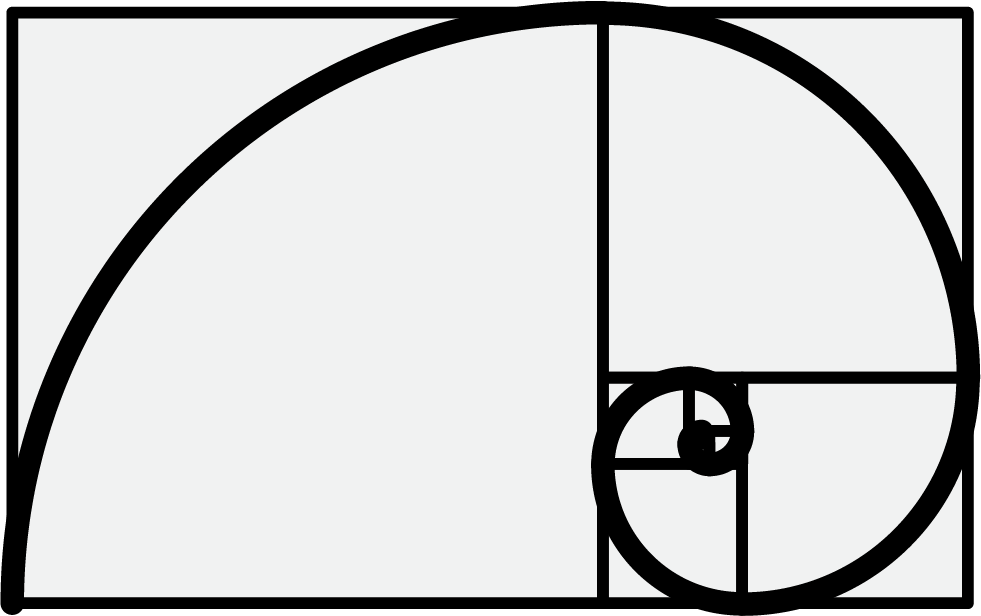
\includegraphics[height=0.75cm]{../../AAA_template_latex_settings/pwr-control_logo_doc.png}}
\lfoot{\href{https://github.com/pwr-control}{\color{black} pwr-control}}
\cfoot{-\ \thepage\ -}
\rfoot{\textit{}}
\renewcommand{\headrulewidth}{0.4pt}
\renewcommand{\footrulewidth}{0.4pt}


\geometry{
	a4paper,
	top    = 2.5cm,
	bottom = 3.0cm,
	left   = 2.5cm,
	right  = 2.5cm
}

\hypersetup{
	colorlinks = true,
	urlcolor   = blue,
	linkcolor  = black,
	citecolor  = black
}

\pagenumbering{gobble}



\usetikzlibrary{decorations.pathreplacing,fit,shapes.geometric}
\usepackage[european,straightvoltages]{circuitikz}
\ctikzset{voltage dir=EF}

\newcommand{\ped}[1]{_{\mathrm{#1}}}
\newcommand{\code}[1]{\texttt{#1}}
\renewcommand{\tabularxcolumn}[1]{>{\raggedright\arraybackslash}p{#1}}
\setlength{\emergencystretch}{3em}

% ---------------- document metadata (read by the title page) ----------------
\newcommand{\DocCategory}{Technical Design Note}
\newcommand{\DocField}{Power Electronics and Control Systems}

\newcommand{\DocTitle}{%
	{\fontsize{20}{24}\selectfont\bfseries CLLC-DCX isolated DC/DC stage} \\[16pt]
	{\fontsize{16}{20}\selectfont\bfseries \SI{800}{\volt} / \SI{800}{\volt}, \SI{50}{\kilo\watt}, \SI{50}{\kilo\hertz}: sizing, simulation model and library block}
}

\newcommand{\DocSubtitle}{%
	Isolated DC transformer of the solid state transformer module, with the \SI{35}{\kilo\hertz} variant \SI{790}{\volt} to \SI{700}{\volt}.
}

\newcommand{\DocAuthor}{Davide Bagnara}
\newcommand{\DocRevision}{00}
\newcommand{\DocDate}{October 2026}

\newcommand{\DocAbstract}{%
	The solid state transformer (SST) module of the \code{solid-state-transformers} repository couples a \SI{800}{\volt} battery bus to a single-phase T-type inverter through a galvanically isolated DC/DC stage. This note documents that stage: a bidirectional CLLC resonant converter operated as a DC transformer (DCX), that is at fixed \SI{50}{\percent} duty, with the switching frequency a little below the series resonance and the rectifying bridge driven as a synchronous rectifier by the sign of its own current. The sizing of the \SI{800}{\volt} / \SI{800}{\volt}, \SI{50}{\kilo\watt}, \SI{50}{\kilo\hertz} stage is derived step by step (operating point, resonant tank and magnetizing inductance, transformer, semiconductors, DC links, loss budget), together with the reasons why the stage is left in open loop. The \SI{35}{\kilo\hertz} variant \SI{790}{\volt} to \SI{700}{\volt}, kept in the repository next to the specification, is documented in the same way and the origin of its numbers is explained. The second part describes the Simscape simulation bench of the repository (power flow modes, switch model, numerical settings and the numerical damping of the fixed-step solver) and the compact library block \code{cllc\_dcx} of \code{pwr-control/library}, a single Simscape component for the power stage and a single MATLAB Function for modulator, synchronous rectifiers and control, with its ports, measurement and gate vectors, control log and parameter structure.
}

\newcommand{\RevisionHistory}{%
	00 & October 2026 & First issue: sizing of the \SI{50}{\kilo\hertz} stage and of the \SI{35}{\kilo\hertz} variant, simulation bench, library block. & \DocAuthor \\
}

\newcommand{\MetaLabelA}{Project Repository}
\newcommand{\MetaValueAUrl}{https://github.com/pwr-control/solid-state-transformers.git}
\newcommand{\MetaValueALabel}{solid-state-transformers.git}

\newcommand{\MetaLabelB}{Framework}
\newcommand{\MetaValueB}{MATLAB/Simulink/Simscape}

\begin{document}

% =============================================================
%  pwr-control LaTeX template - FRONTESPIZIO
%
%  Da richiamare come prima istruzione dopo \begin{document}:
%      % =============================================================
%  pwr-control LaTeX template - FRONTESPIZIO
%
%  Da richiamare come prima istruzione dopo \begin{document}:
%      % =============================================================
%  pwr-control LaTeX template - FRONTESPIZIO
%
%  Da richiamare come prima istruzione dopo \begin{document}:
%      \input{../../AAA_template_latex_settings/titlepage}
%
%  Il documento deve definire prima di \begin{document}:
%      \DocCategory   categoria del documento
%      \DocField      area tecnica
%      \DocTitle      titolo (una o due righe)
%      \DocSubtitle   sottotitolo
%      \DocAuthor     autore/i, separati da virgola
%      \DocRevision   numero di revisione corrente (es. 00)
%      \DocDate       data della revisione corrente
%      \DocAbstract   abstract
%      \RevisionHistory  righe della tabella di revisione, nel formato
%                        Rev. & Date & Description & Authors \\
%      \MetaLabelA \MetaValueAUrl \MetaValueALabel
%      \MetaLabelB \MetaValueB
% =============================================================

\providecommand{\DocCategory}{Technical Research Report}
\providecommand{\DocField}{Power Electronics and Control Systems}
\providecommand{\DocSubtitle}{}
\providecommand{\DocRevision}{00}
\providecommand{\DocAbstract}{}
\providecommand{\RevisionHistory}{%
	\DocRevision & \DocDate & First issue. & \DocAuthor \\
}

\titlepage

% ---- Intestazione centrata ----
\begin{center}
	{\Large\scshape \DocCategory}\\[8pt]
	{\large\scshape \DocField}
\end{center}

\vspace{30pt plus 4pt minus 14pt}
\noindent\rule{\linewidth}{0.8pt}

% ---- Titolo ----
\begin{center}
	\DocTitle
\end{center}

\vspace{4pt}
\noindent\rule{\linewidth}{2.2pt}

% ---- Sottotitolo ----
\begin{center}
	\begin{onehalfspace}
		{\large\itshape \DocSubtitle}
	\end{onehalfspace}
\end{center}

% ---- Authors / Revision / Date ----
\vspace{30pt plus 4pt minus 14pt}

\noindent
\begin{minipage}[t]{0.46\linewidth}
	\raggedright
	\textbf{Authors:}\\[2pt]
	\DocAuthor
\end{minipage}%
\hfill
\begin{minipage}[t]{0.22\linewidth}
	\centering
	\textbf{Revision:}\\[2pt]
	\DocRevision
\end{minipage}%
\hfill
\begin{minipage}[t]{0.30\linewidth}
	\raggedleft
	\textbf{Date:}\\[2pt]
	\DocDate
\end{minipage}

\vspace{10pt}
\noindent\rule{\linewidth}{0.8pt}

% ---- Abstract ----
\vspace{24pt plus 4pt minus 12pt}

\begin{center}
	\begin{minipage}{0.88\linewidth}
		\footnotesize
		\begin{onehalfspace}
			\textbf{Abstract:} \DocAbstract
		\end{onehalfspace}
	\end{minipage}
\end{center}

\vfill

% ---- Revision history ----
\begin{center}
	\begin{minipage}{0.96\linewidth}
		\centering
		{\footnotesize\scshape Revision history}\\[6pt]
		{\footnotesize
			\begin{tabular}{@{}cl>{\raggedright\arraybackslash}p{0.36\linewidth}>{\raggedright\arraybackslash}p{0.28\linewidth}@{}}
				\toprule
				\textbf{Rev.} & \textbf{Date} & \textbf{Description} & \textbf{Authors} \\
				\midrule
				\RevisionHistory
				\bottomrule
			\end{tabular}}
	\end{minipage}
\end{center}

\vspace{18pt plus 4pt minus 10pt}

% ---- Metadati in fondo ----
\noindent
\begin{tabular}{@{} r @{\quad} l @{}}
	\textsc{\MetaLabelA:} & {\href{\MetaValueAUrl}{\MetaValueALabel}} \\[3pt]
	\textsc{\MetaLabelB:} & {\MetaValueB}       \\[3pt]
\end{tabular}

% =============================================================
%  Fine frontespizio
% =============================================================
\newpage
\pagenumbering{arabic}
\setcounter{page}{1}

%
%  Il documento deve definire prima di \begin{document}:
%      \DocCategory   categoria del documento
%      \DocField      area tecnica
%      \DocTitle      titolo (una o due righe)
%      \DocSubtitle   sottotitolo
%      \DocAuthor     autore/i, separati da virgola
%      \DocRevision   numero di revisione corrente (es. 00)
%      \DocDate       data della revisione corrente
%      \DocAbstract   abstract
%      \RevisionHistory  righe della tabella di revisione, nel formato
%                        Rev. & Date & Description & Authors \\
%      \MetaLabelA \MetaValueAUrl \MetaValueALabel
%      \MetaLabelB \MetaValueB
% =============================================================

\providecommand{\DocCategory}{Technical Research Report}
\providecommand{\DocField}{Power Electronics and Control Systems}
\providecommand{\DocSubtitle}{}
\providecommand{\DocRevision}{00}
\providecommand{\DocAbstract}{}
\providecommand{\RevisionHistory}{%
	\DocRevision & \DocDate & First issue. & \DocAuthor \\
}

\titlepage

% ---- Intestazione centrata ----
\begin{center}
	{\Large\scshape \DocCategory}\\[8pt]
	{\large\scshape \DocField}
\end{center}

\vspace{30pt plus 4pt minus 14pt}
\noindent\rule{\linewidth}{0.8pt}

% ---- Titolo ----
\begin{center}
	\DocTitle
\end{center}

\vspace{4pt}
\noindent\rule{\linewidth}{2.2pt}

% ---- Sottotitolo ----
\begin{center}
	\begin{onehalfspace}
		{\large\itshape \DocSubtitle}
	\end{onehalfspace}
\end{center}

% ---- Authors / Revision / Date ----
\vspace{30pt plus 4pt minus 14pt}

\noindent
\begin{minipage}[t]{0.46\linewidth}
	\raggedright
	\textbf{Authors:}\\[2pt]
	\DocAuthor
\end{minipage}%
\hfill
\begin{minipage}[t]{0.22\linewidth}
	\centering
	\textbf{Revision:}\\[2pt]
	\DocRevision
\end{minipage}%
\hfill
\begin{minipage}[t]{0.30\linewidth}
	\raggedleft
	\textbf{Date:}\\[2pt]
	\DocDate
\end{minipage}

\vspace{10pt}
\noindent\rule{\linewidth}{0.8pt}

% ---- Abstract ----
\vspace{24pt plus 4pt minus 12pt}

\begin{center}
	\begin{minipage}{0.88\linewidth}
		\footnotesize
		\begin{onehalfspace}
			\textbf{Abstract:} \DocAbstract
		\end{onehalfspace}
	\end{minipage}
\end{center}

\vfill

% ---- Revision history ----
\begin{center}
	\begin{minipage}{0.96\linewidth}
		\centering
		{\footnotesize\scshape Revision history}\\[6pt]
		{\footnotesize
			\begin{tabular}{@{}cl>{\raggedright\arraybackslash}p{0.36\linewidth}>{\raggedright\arraybackslash}p{0.28\linewidth}@{}}
				\toprule
				\textbf{Rev.} & \textbf{Date} & \textbf{Description} & \textbf{Authors} \\
				\midrule
				\RevisionHistory
				\bottomrule
			\end{tabular}}
	\end{minipage}
\end{center}

\vspace{18pt plus 4pt minus 10pt}

% ---- Metadati in fondo ----
\noindent
\begin{tabular}{@{} r @{\quad} l @{}}
	\textsc{\MetaLabelA:} & {\href{\MetaValueAUrl}{\MetaValueALabel}} \\[3pt]
	\textsc{\MetaLabelB:} & {\MetaValueB}       \\[3pt]
\end{tabular}

% =============================================================
%  Fine frontespizio
% =============================================================
\newpage
\pagenumbering{arabic}
\setcounter{page}{1}

%
%  Il documento deve definire prima di \begin{document}:
%      \DocCategory   categoria del documento
%      \DocField      area tecnica
%      \DocTitle      titolo (una o due righe)
%      \DocSubtitle   sottotitolo
%      \DocAuthor     autore/i, separati da virgola
%      \DocRevision   numero di revisione corrente (es. 00)
%      \DocDate       data della revisione corrente
%      \DocAbstract   abstract
%      \RevisionHistory  righe della tabella di revisione, nel formato
%                        Rev. & Date & Description & Authors \\
%      \MetaLabelA \MetaValueAUrl \MetaValueALabel
%      \MetaLabelB \MetaValueB
% =============================================================

\providecommand{\DocCategory}{Technical Research Report}
\providecommand{\DocField}{Power Electronics and Control Systems}
\providecommand{\DocSubtitle}{}
\providecommand{\DocRevision}{00}
\providecommand{\DocAbstract}{}
\providecommand{\RevisionHistory}{%
	\DocRevision & \DocDate & First issue. & \DocAuthor \\
}

\titlepage

% ---- Intestazione centrata ----
\begin{center}
	{\Large\scshape \DocCategory}\\[8pt]
	{\large\scshape \DocField}
\end{center}

\vspace{30pt plus 4pt minus 14pt}
\noindent\rule{\linewidth}{0.8pt}

% ---- Titolo ----
\begin{center}
	\DocTitle
\end{center}

\vspace{4pt}
\noindent\rule{\linewidth}{2.2pt}

% ---- Sottotitolo ----
\begin{center}
	\begin{onehalfspace}
		{\large\itshape \DocSubtitle}
	\end{onehalfspace}
\end{center}

% ---- Authors / Revision / Date ----
\vspace{30pt plus 4pt minus 14pt}

\noindent
\begin{minipage}[t]{0.46\linewidth}
	\raggedright
	\textbf{Authors:}\\[2pt]
	\DocAuthor
\end{minipage}%
\hfill
\begin{minipage}[t]{0.22\linewidth}
	\centering
	\textbf{Revision:}\\[2pt]
	\DocRevision
\end{minipage}%
\hfill
\begin{minipage}[t]{0.30\linewidth}
	\raggedleft
	\textbf{Date:}\\[2pt]
	\DocDate
\end{minipage}

\vspace{10pt}
\noindent\rule{\linewidth}{0.8pt}

% ---- Abstract ----
\vspace{24pt plus 4pt minus 12pt}

\begin{center}
	\begin{minipage}{0.88\linewidth}
		\footnotesize
		\begin{onehalfspace}
			\textbf{Abstract:} \DocAbstract
		\end{onehalfspace}
	\end{minipage}
\end{center}

\vfill

% ---- Revision history ----
\begin{center}
	\begin{minipage}{0.96\linewidth}
		\centering
		{\footnotesize\scshape Revision history}\\[6pt]
		{\footnotesize
			\begin{tabular}{@{}cl>{\raggedright\arraybackslash}p{0.36\linewidth}>{\raggedright\arraybackslash}p{0.28\linewidth}@{}}
				\toprule
				\textbf{Rev.} & \textbf{Date} & \textbf{Description} & \textbf{Authors} \\
				\midrule
				\RevisionHistory
				\bottomrule
			\end{tabular}}
	\end{minipage}
\end{center}

\vspace{18pt plus 4pt minus 10pt}

% ---- Metadati in fondo ----
\noindent
\begin{tabular}{@{} r @{\quad} l @{}}
	\textsc{\MetaLabelA:} & {\href{\MetaValueAUrl}{\MetaValueALabel}} \\[3pt]
	\textsc{\MetaLabelB:} & {\MetaValueB}       \\[3pt]
\end{tabular}

% =============================================================
%  Fine frontespizio
% =============================================================
\newpage
\pagenumbering{arabic}
\setcounter{page}{1}


\tableofcontents
\listoffigures
\listoftables
\newpage

\begin{onehalfspace}

% =============================================================
\section*{Nomenclature}
\addcontentsline{toc}{section}{Nomenclature}
\label{sec:nomenclature}

\rowcolors{2}{tableShade}{white}
\begin{longtable}{@{} l p{0.72\linewidth} @{}}
	\toprule
	\textbf{Symbol} & \textbf{Meaning} \\
	\midrule
	\endfirsthead
	\toprule
	\textbf{Symbol} & \textbf{Meaning} \\
	\midrule
	\endhead
	\bottomrule
	\endfoot
	\bottomrule
	\endlastfoot
	$u\ped{1}$, $u\ped{2}$ & DC voltages of side 1 (battery bus, \SI{800}{\volt}) and of side 2 (isolated DC link of the inverter) \\
	$i\ped{dc1}$, $i\ped{dc2}$ & DC currents of the two sides; $i\ped{dc1}$ positive into the stage, $i\ped{dc2}$ positive out of it \\
	$P$ & transferred power, \SI{50}{\kilo\watt} nominal \\
	$n = n\ped{1}/n\ped{2}$ & turns ratio of the transformer ($11:11$ for the \SI{50}{\kilo\hertz} stage, $9:8$ for the \SI{35}{\kilo\hertz} variant) \\
	$f\ped{s}$, $\omega\ped{s}$ & switching frequency of the bridges and its angular value \\
	$f\ped{r}$, $\omega\ped{r}$ & series resonance of one side of the tank, $\omega\ped{r} = 1/\sqrt{L\ped{r1} C\ped{r1}}$ \\
	$f\ped{n} = f\ped{s}/f\ped{r}$ & normalized switching frequency, $0.95$ in both designs \\
	$L\ped{r1}$, $C\ped{r1}$ & resonant inductance and capacitance of side 1 (leakage plus discrete inductor) \\
	$L\ped{r2}$, $C\ped{r2}$ & resonant inductance and capacitance of side 2, $L\ped{r2} = L\ped{r1}/n^2$, $C\ped{r2} = n^2 C\ped{r1}$ \\
	$L\ped{m}$ & magnetizing inductance of the transformer, referred to side 1 \\
	$L\ped{n} = L\ped{m}/L\ped{r1}$ & inductance ratio of the tank \\
	$Z\ped{0} = \sqrt{L\ped{r1}/C\ped{r1}}$ & characteristic impedance of one side of the tank \\
	$R\ped{ac} = 8 n^2 u\ped{2}^2/(\pi^2 P)$ & first-harmonic (FHA) load resistance seen from side 1 \\
	$Q = Z\ped{0}/R\ped{ac}$ & quality factor of the tank at the operating point \\
	$M$ & FHA voltage gain of the tank, $M = n\,u\ped{2}/u\ped{1}$ \\
	$X(f\ped{s})$ & series reactance of the whole tank at the switching frequency, referred to side 1 \\
	$\varphi$ & phase displacement of bridge 2 after bridge 1 (positive when bridge 2 lags) \\
	$i\ped{r1}$, $i\ped{r2}$ & tank currents of side 1 and side 2 \\
	$I\ped{1pk}$, $I\ped{1rms}$ & peak and rms value of the resonant current of side 1 \\
	$I\ped{m}$ & peak of the magnetizing current \\
	$u\ped{b1}$, $u\ped{b2}$ & output voltages of the two full bridges (square waves of amplitude $u\ped{1}$, $u\ped{2}$) \\
	$u\ped{cr1}$, $u\ped{cr2}$ & voltages across the two resonant capacitors \\
	$C\ped{oss}$ & output capacitance of one switch, energy related \\
	$t\ped{d}$ & dead time of the driving bridge, \SI{300}{\nano\second} \\
	$t\ped{c}$ & step of the Simscape local solver and sample time of the control block \\
	$R\ped{num}$ & extra series resistance introduced by the Backward Euler method at the switching frequency \\
	$C\ped{dc1}$, $L\ped{dc1}$ & DC-link capacitor and DC choke of side 1 (the same on side 2 with index 2) \\
	DCX & DC transformer: a resonant converter run at fixed frequency and fixed \SI{50}{\percent} duty \\
	SR & synchronous rectifier (the bridge that rectifies, driven by the sign of its own current) \\
	FHA & first-harmonic approximation \\
	ZVS & zero-voltage switching \\
\end{longtable}
\addtocounter{table}{-1}
\rowcolors{1}{white}{white}

% =============================================================
\section{Introduction and scope}
\label{sec:intro}

The solid state transformer studied in \cite{sst_doc} is a chain of modules, each one made of an isolated DC/DC stage and of a single-phase inverter; the DC/DC stages share the battery bus and the inverters are connected in series on the AC side. The repository \code{solid-state-transformers} \cite{sst_repo} keeps, in the folder \path{theory_analysis_solid_state_transformer}, the simulation bench of one module built around the two stages documented here and in \cite{spinv_doc}: the CLLC resonant converter used as a DC transformer (this note) and the single-phase T-type inverter with its grid-tied control.

Figure~\ref{fig:module} places the DCX in the module. Side 1 of the DCX is the \SI{800}{\volt} battery bus of the module; side 2 is the galvanically isolated \SI{800}{\volt} DC link of the T-type inverter. The DCX has three tasks and no other: it provides the galvanic isolation that lets the inverters be stacked in series, it carries \SI{50}{\kilo\watt} in both directions, and it keeps the ratio $u\ped{2}/u\ped{1}$ fixed at $1/n$. It does not regulate: the voltage of the inverter DC link follows the battery, and the current drawn from it is set by the inverter. This is what the term DCX means \cite{jung2013, huang2010}, and it is the reason why the stage can run at the optimum of the resonant tank at any load, with zero-voltage switching of the driving bridge and almost zero-current switching of the rectifying one.

\begin{figure}[H]
	\centering
	\begin{tikzpicture}[font=\footnotesize, >=Latex,
		blk/.style={draw, thick, rounded corners=2pt, minimum height=1.4cm, align=center, fill=blue!4},
		lnk/.style={draw, thick, rounded corners=2pt, minimum height=1.4cm, align=center, fill=gray!8, dashed}]
		\node[lnk] (bat) {battery pack\\\SI{800}{\volt}};
		\node[blk, right=0.7cm of bat, minimum width=2.8cm, fill=orange!12] (dcx) {CLLC-DCX\\\SI{800}{\volt} / \SI{800}{\volt}\\\SI{50}{\kilo\watt}, \SI{50}{\kilo\hertz}};
		\node[lnk, right=0.7cm of dcx] (dcl) {isolated DC link\\\SI{800}{\volt}};
		\node[blk, right=0.7cm of dcl, minimum width=2.6cm] (inv) {T-type inverter\\single phase\\\SI{4}{\kilo\hertz} PWM};
		\node[lnk, right=0.7cm of inv] (ac) {AC output\\\SI{398}{\volt} rms};
		\draw[<->, thick] (bat) -- (dcx) node[midway, above, font=\scriptsize] {side 1};
		\draw[<->, thick] (dcx) -- (dcl) node[midway, above, font=\scriptsize] {side 2};
		\draw[<->, thick] (dcl) -- (inv);
		\draw[<->, thick] (inv) -- (ac);
		\draw[decorate, decoration={brace, amplitude=5pt, mirror}] ([yshift=-3mm]bat.south west) -- ([yshift=-3mm]ac.south east) node[midway, below=5pt] {one module of the SST};
	\end{tikzpicture}
	\captionsetup{width=0.9\textwidth, font=small}
	\caption[The DCX in the SST module.]{The DCX in the SST module: side 1 on the battery bus, side 2 on the isolated DC link of the single-phase inverter. The DCX fixes the ratio of the two voltages; the inverter sets the power. The bench of \cite{sst_repo} puts two modules in series on the AC side.}
	\label{fig:module}
\end{figure}

The note has two parts. Sections~\ref{sec:sizing} and~\ref{sec:variant} are the sizing: the \SI{800}{\volt} / \SI{800}{\volt}, \SI{50}{\kilo\watt}, \SI{50}{\kilo\hertz} stage that is the specification of the module, and the \SI{35}{\kilo\hertz} variant \SI{790}{\volt} to \SI{700}{\volt} that the repository keeps next to it. Sections~\ref{sec:model} and~\ref{sec:library} are the models: the Simscape bench of the repository, built with the discrete blocks of the library, and the compact block \code{cllc\_dcx} of \code{pwr-control/library} \cite{library_repo}, which packs the whole stage into two nonvirtual blocks for the SST bench. The numbers of this note are those of the parameter files of the two repositories (\code{private/cllc\_dcx\_param.m} of each bench folder, \code{cllc\_dcx\_param\_example.m} and \code{cllc\_dcx\_param\_example\_35kHz.m} of the library); the analytic figures are produced by the script \code{py/cllc\_dcx\_figures.py} of this folder from the same numbers. At the time of writing no simulation run of the DCX is saved in the repository: Section~\ref{sec:checks} lists what the first runs have to compare with the sizing.

% =============================================================
\section{Sizing of the \SI{800}{\volt} / \SI{800}{\volt}, \SI{50}{\kilo\watt}, \SI{50}{\kilo\hertz} stage}
\label{sec:sizing}

\subsection{Operating point}
\label{sec:op}

Table~\ref{tab:op} is the operating point. Both DC links are at \SI{800}{\volt}, so the transformer is $1:1$ and the same SiC module is used on both bridges; the base current is $i\ped{dc1} = P/u\ped{1} = \SI{62.5}{\ampere}$ on both sides. The switching frequency is \SI{50}{\kilo\hertz}, the highest value at which the transformer still fits in one layer of litz wire per winding on a stack of standard ferrite U-cores (Section~\ref{sec:transformer}) and at which the \SI{300}{\nano\second} dead time of the SiC modules is still a small fraction of the period (\ang{5.4} of the fundamental).

\begin{table}[H]
	\centering
	\captionsetup{width=0.9\textwidth, font=small}
	\caption{Operating point of the DCX.}
	\label{tab:op}
	\rowcolors{2}{tableShade}{white}
	\begin{tabularx}{0.95\textwidth}{@{} l l X @{}}
		\toprule
		\textbf{Quantity} & \textbf{Value} & \textbf{Note} \\
		\midrule
		DC voltage, side 1 ($u\ped{1}$) & \SI{800}{\volt} & battery bus of the module \\
		DC voltage, side 2 ($u\ped{2}$) & \SI{800}{\volt} & isolated DC link of the T-type inverter, $u\ped{2} = u\ped{1}/n$ \\
		Turns ratio & $11:11$ & one layer per winding, Section~\ref{sec:transformer} \\
		Nominal power & \SI{50}{\kilo\watt} & both directions \\
		DC current, both sides & \SI{62.5}{\ampere} & base of the pu system of the model \\
		Switching frequency $f\ped{s}$ & \SI{50}{\kilo\hertz} & both bridges, \SI{50}{\percent} duty \\
		Series resonance $f\ped{r}$ & \SI{52.6}{\kilo\hertz} & $f\ped{n} = f\ped{s}/f\ped{r} = 0.95$ \\
		Dead time $t\ped{d}$ & \SI{300}{\nano\second} & driving bridge, ZVS with the magnetizing current \\
		Semiconductors & Wolfspeed CAB006M12GM3 & \SI{1200}{\volt} SiC half-bridge modules, both bridges \\
		Control & open loop (DCX) & bridge 2 synchronous rectifier on $i\ped{r2}$ \\
		\bottomrule
	\end{tabularx}
	\rowcolors{1}{white}{white}
\end{table}

\subsection{Principle of operation and first-harmonic gain}
\label{sec:principle}

The CLLC converter \cite{jung2013} is the bidirectional form of the LLC converter \cite{yang2002, huang2010}: two full bridges and a transformer whose leakage, completed by a discrete inductor, resonates with a series capacitor on each side (Figure~\ref{fig:bench}). The two tanks are symmetrical when referred to the same side, $L\ped{r2} = L\ped{r1}/n^2$ and $C\ped{r2} = n^2 C\ped{r1}$, so the converter has the same resonance and the same gain in both directions of the power flow.

With the first-harmonic approximation (FHA) \cite{steigerwald1988} the load is the resistance $R\ped{ac} = 8 n^2 u\ped{2}^2/(\pi^2 P)$ and the gain of the tank, referred to the primary, is
\begin{equation}
	M(f\ped{n}) = \frac{n\,u\ped{2}}{u\ped{1}} =
	\frac{1}{\sqrt{\left[1 + \dfrac{1}{L\ped{n}}\left(1 - \dfrac{1}{f\ped{n}^2}\right)\right]^2 + Q^2 \left(f\ped{n} - \dfrac{1}{f\ped{n}}\right)^2}},
	\qquad Q = \frac{Z\ped{0}}{R\ped{ac}},\quad L\ped{n} = \frac{L\ped{m}}{L\ped{r1}},
	\label{eq:gain}
\end{equation}
which is the gain of the LLC tank with the load resistance in series with the second resonant branch; the exact FHA network with both branches, used for Figure~\ref{fig:gain}, differs from Eq.~\eqref{eq:gain} by less than \SI{0.1}{\percent} around $f\ped{n} = 1$ at the values of $Q$ and $L\ped{n}$ of this design. At $f\ped{n} = 1$ the gain is one at any load: this is the DCX point. Figure~\ref{fig:gain} shows the gain for three loads with the tank of Section~\ref{sec:tank}: between \SI{10}{\percent} and \SI{100}{\percent} of the load the gain at $f\ped{n} = 0.95$ stays within \SI{0.3}{\percent} of one, so the open-loop stage is a stiff DC transformer. The input impedance of the tank is almost resistive at full load (\ang{0.2} at \SI{100}{\percent}, \ang{7} at \SI{50}{\percent}) and becomes inductive at light load (\ang{39} at \SI{10}{\percent}) because of the magnetizing branch: the bridge current never leads the voltage, which is the condition for ZVS.

\begin{figure}[H]
	\centering
	\begin{tikzpicture}
		\begin{axis}[
			width=0.82\linewidth, height=6.4cm,
			xlabel={$f\ped{n} = f\ped{s}/f\ped{r}$}, ylabel={gain $M = n\,u\ped{2}/u\ped{1}$},
			xmin=0.5, xmax=1.5, ymin=0.9, ymax=1.1,
			grid=major, grid style={gray!25},
			legend pos=north east, legend style={font=\footnotesize, fill=white},
			tick label style={font=\footnotesize}, label style={font=\small}]
			\addplot[thick, blue!70!black] table[x=fn, y=M10] {figures/fha_gain_50kHz.dat};
			\addlegendentry{$Q = 0.04$ (\SI{10}{\percent} load)}
			\addplot[thick, orange!80!black] table[x=fn, y=M50] {figures/fha_gain_50kHz.dat};
			\addlegendentry{$Q = 0.19$ (\SI{50}{\percent} load)}
			\addplot[thick, red!70!black] table[x=fn, y=M100] {figures/fha_gain_50kHz.dat};
			\addlegendentry{$Q = 0.38$ (full load)}
			\draw[dashed, gray] (axis cs:0.95,0.9) -- (axis cs:0.95,1.1);
			\node[font=\footnotesize, anchor=south east, fill=white, inner sep=1pt] at (axis cs:0.94,0.905) {$f\ped{n} = 0.95$};
		\end{axis}
	\end{tikzpicture}
	\captionsetup{width=0.85\textwidth, font=small}
	\caption[First-harmonic gain of the CLLC tank.]{First-harmonic gain of the tank of Section~\ref{sec:tank} ($L\ped{n} = 33$) for three loads, exact FHA network with both resonant branches (\code{figures/fha\_gain\_50kHz.dat}). The working point $f\ped{n} = 0.95$ is marked.}
	\label{fig:gain}
\end{figure}

\noindent\textbf{Why $f\ped{r}$ a little above $f\ped{s}$.} With $f\ped{s} < f\ped{r}$ the resonant half sine of the current ends before the end of the half period: the rectifying bridge turns off at zero current, and in the remaining interval the driving bridge carries the magnetizing current only, which is what commutates it with ZVS. With $f\ped{r} = \SI{52.6}{\kilo\hertz}$ the half sine lasts \SI{9.5}{\micro\second} of the \SI{10}{\micro\second} half period and still ends before the commutation with the tolerances of $L\ped{r}$ and $C\ped{r}$ ($f\ped{r} \pm \SI{7}{\percent}$ for $C\ped{r} \pm \SI{5}{\percent}$ and $L\ped{r} \pm \SI{10}{\percent}$). A larger gap would not be a DCX any more: the current becomes more peaked, the conduction losses and the voltage on $C\ped{r}$ grow, and the gain starts to move with the load. Above resonance ($f\ped{n} > 1$) the rectifier would be turned off while still carrying current, losing the soft turn-off.

\subsection{Why the DCX does not regulate}
\label{sec:noreg}

The phase displacement $\varphi$ between the two bridges, which is the control variable of the dual active bridge \cite{dedoncker1991, krismer2010}, is available in the modulator of the model, and the question whether to close a loop on it comes up naturally. With the fundamentals, the power from bridge 1 to bridge 2 is
\begin{equation}
	P(\varphi) \simeq \frac{U\ped{1} \, n U\ped{2}}{2\,\abs{X(f\ped{s})}} \sin\varphi
	\qquad\text{with}\qquad U\ped{1} = \frac{4}{\pi} u\ped{1},\quad U\ped{2} = \frac{4}{\pi} u\ped{2},
	\label{eq:pphi}
\end{equation}
where $X(f\ped{s}) = 2\left(\omega\ped{s} L\ped{r1} - 1/(\omega\ped{s} C\ped{r1})\right)$ is the series reactance of the whole tank referred to side 1, with $L\ped{m}$ neglected. At $f\ped{n} = 0.95$ the tank of Section~\ref{sec:tank} gives $X(f\ped{s}) = \SI{-0.81}{\ohm}$, small and capacitive, so that $P \simeq \SI{640}{\kilo\watt}\,\sin\varphi$: the nominal \SI{50}{\kilo\watt} corresponds to $\varphi = \ang{4.5}$ (Figure~\ref{fig:pphi}), and the dead time alone is \ang{5.4}. Three facts follow.

\begin{enumerate}[nosep]
	\item The stage is extremely stiff: a few degrees of phase move tens of kilowatts, and the gain of a phase-shift loop would be about \SI{13}{pu/rad} of DC current. Any control on $\varphi$ needs small gains and the current is then set by the bridge, not by the loop (Section~\ref{sec:ctrl_chain}).
	\item Since $X(f\ped{s}) < 0$, a positive $\varphi$ (bridge 2 lagging) would carry power from side 2 to side 1, opposite to the inductive case of the DAB; the sign of the reactance has to enter the control law.
	\item When bridge 2 is driven by a phase-shifted PWM instead of following its own current, the rectifier switches with current at the dead time and the tank is forced into capacitive operation: the natural operation of the CLLC near resonance is incompatible with a regulated phase.
\end{enumerate}

\noindent The DCX is therefore left in open loop (mode~0 of the control, Section~\ref{sec:ctrl_chain}): bridge 1 at \SI{50}{\percent} duty, bridge 2 as a synchronous rectifier driven by the sign of $i\ped{r2}$. The power and the direction of the flow are set by the stages around it, as in Figure~\ref{fig:module}; the voltage of side 2 follows $u\ped{1}/n$ minus the drop on an equivalent resistance of about \SI{43}{\milli\ohm} (Section~\ref{sec:losses}). The current and voltage loops of the library block (modes 1 and 2) are kept as an option for other uses of the same stage, not for the SST.

\begin{figure}[H]
	\centering
	\begin{tikzpicture}
		\begin{axis}[
			width=0.72\linewidth, height=5.6cm,
			xlabel={phase displacement $\varphi$ [\si{\degree}]}, ylabel={$P(\varphi)$ [\si{\kilo\watt}]},
			xmin=0, xmax=12, ymin=0, ymax=140,
			grid=major, grid style={gray!25},
			legend pos=north west, legend style={font=\footnotesize, fill=white},
			tick label style={font=\footnotesize}, label style={font=\small}]
			\addplot[thick, red!70!black, domain=0:12, samples=121] {637*sin(x)};
			\addlegendentry{\SI{50}{\kilo\hertz} stage, $X = \SI{-0.81}{\ohm}$}
			\addplot[thick, blue!70!black, dashed, domain=0:12, samples=121] {665*sin(x)};
			\addlegendentry{\SI{35}{\kilo\hertz} variant, $X = \SI{-0.76}{\ohm}$}
			\draw[dashed, gray] (axis cs:0,50) -- (axis cs:4.5,50) -- (axis cs:4.5,0);
			\node[font=\footnotesize, anchor=south west] at (axis cs:4.6,52) {\SI{50}{\kilo\watt} at \ang{4.5}};
			\draw[dotted, gray!80!black, thick] (axis cs:5.4,0) -- (axis cs:5.4,140);
			\node[font=\footnotesize, anchor=north west, rotate=90] at (axis cs:5.5,60) {dead time \SI{300}{\nano\second}};
		\end{axis}
	\end{tikzpicture}
	\captionsetup{width=0.85\textwidth, font=small}
	\caption[Power against phase displacement.]{Power against phase displacement of the two bridges with the fundamentals, Eq.~\eqref{eq:pphi}: the nominal power is reached at \ang{4.5}, less than the \ang{5.4} of the dead time at \SI{50}{\kilo\hertz}. The stage cannot be regulated through $\varphi$ with the bridges in PWM.}
	\label{fig:pphi}
\end{figure}

\subsection{Resonant tank and magnetizing inductance}
\label{sec:tank}

\noindent\textbf{Currents.} With $f\ped{s} < f\ped{r}$ each half period carries the charge $i\ped{dc1}/(2 f\ped{s})$ in a half sine of period $1/f\ped{r}$:
\begin{equation}
	I\ped{1pk} = \frac{\pi}{2}\,\frac{i\ped{dc1}}{f\ped{n}} = \SI{103}{\ampere}, \qquad
	I\ped{1rms} = I\ped{1pk} \sqrt{\frac{f\ped{n}}{2}} = \SI{71.2}{\ampere},
	\label{eq:currents}
\end{equation}
\SI{71.5}{\ampere} rms and \SI{113}{\ampere} peak with the magnetizing triangle added. Side 2 carries the same current ($n = 1$).

\noindent\textbf{Magnetizing inductance.} The magnetizing current must charge and discharge the output capacitances of one leg of the driving bridge within the dead time. The charge of a leg is $Q\ped{leg} = 2 C\ped{oss} u\ped{1} = 2 \cdot \SI{0.79}{\nano\farad} \cdot \SI{800}{\volt} = \SI{1.26}{\micro\coulomb}$, so the minimum peak is $Q\ped{leg}/t\ped{d} = \SI{4.2}{\ampere}$. With margin, $I\ped{m} = \SI{10}{\ampere}$:
\begin{equation}
	L\ped{m} = \frac{u\ped{1}}{4 I\ped{m} f\ped{s}} = \frac{800}{4 \cdot 10 \cdot 50000} = \SI{400}{\micro\henry},
	\qquad t\ped{ZVS} = \frac{2 C\ped{oss} u\ped{1}}{I\ped{m}} = \SI{126}{\nano\second} < t\ped{d} = \SI{300}{\nano\second}.
	\label{eq:lm}
\end{equation}
The upper bound for the ZVS is $L\ped{m} \le t\ped{d}/(8 f\ped{s} C\ped{oss}) = \SI{950}{\micro\henry}$; with $I\ped{m} = \SI{10}{\ampere}$ the leg capacitance may grow up to $I\ped{m} t\ped{d}/u\ped{1} = \SI{3.75}{\nano\farad}$ (snubbers, module paralleling) before the ZVS is lost. $I\ped{m}$ is \SI{14}{\percent} of the resonant peak and its rms value (\SI{5.8}{\ampere}) adds \SI{0.3}{\ampere} to the winding current; the turn-off of the driving bridge happens at $I\ped{m}$ only.

\noindent\textbf{Resonant inductance and capacitance.} $L\ped{r1} = \SI{12}{\micro\henry}$ on side 1: about \SI{4}{\micro\henry} of transformer leakage and the rest a discrete inductor (Section~\ref{sec:transformer}). At $f\ped{r} = \SI{52.6}{\kilo\hertz}$,
\begin{equation}
	C\ped{r1} = \frac{1}{(2\pi f\ped{r})^2 L\ped{r1}} = \SI{0.762}{\micro\farad}, \qquad
	Z\ped{0} = \sqrt{\frac{L\ped{r1}}{C\ped{r1}}} = \SI{3.97}{\ohm},
	\label{eq:tank}
\end{equation}
and with $R\ped{ac} = \SI{10.4}{\ohm}$ the tank has $Q = 0.38$ and $L\ped{n} = 33$. $C\ped{r1}$ is a film capacitor for \SI{71}{\ampere} rms at \SI{50}{\kilo\hertz} and \SI{410}{\volt} peak ($I\ped{1pk}/(\omega\ped{r} C\ped{r1})$); the full-bridge drive keeps the DC component off it. The side 2 tank repeats side 1, $L\ped{r2} = L\ped{r1}/n^2 = \SI{12}{\micro\henry}$ and $C\ped{r2} = n^2 C\ped{r1} = \SI{0.762}{\micro\farad}$, so that the resonance is the same in both power directions and both sides see the same currents and voltages. The small $Q$ and the large $L\ped{n}$ are typical of a DCX \cite{jung2013}: the tank is not asked to provide gain, only to shape the current into a half sine and to make the magnetizing current available for the ZVS.

Figure~\ref{fig:waveforms} shows the idealized waveforms of one side of the tank built from these numbers: the square wave of the bridge, the resonant half sines, the magnetizing triangle and the voltage of the resonant capacitor, which stays constant in the interval between the end of the half sine and the commutation.

\begin{figure}[H]
	\centering
	\begin{tikzpicture}
		\begin{axis}[
			width=0.88\linewidth, height=4.6cm,
			ylabel={[\si{\volt}]}, xmin=0, xmax=40, ymin=-950, ymax=950,
			xticklabels={}, grid=major, grid style={gray!25},
			legend columns=2, legend pos=north east, legend style={font=\footnotesize, fill=white},
			tick label style={font=\footnotesize}, label style={font=\small}]
			\addplot[thick, blue!70!black] table[x=t_us, y=u_b1] {figures/tank_waveforms_50kHz.dat};
			\addlegendentry{$u\ped{b1}$}
			\addplot[thick, red!70!black] table[x=t_us, y=u_cr1] {figures/tank_waveforms_50kHz.dat};
			\addlegendentry{$u\ped{cr1}$}
		\end{axis}
	\end{tikzpicture}

	\begin{tikzpicture}
		\begin{axis}[
			width=0.88\linewidth, height=4.6cm,
			xlabel={$t$ [\si{\micro\second}]}, ylabel={[\si{\ampere}]}, xmin=0, xmax=40, ymin=-130, ymax=130,
			grid=major, grid style={gray!25},
			legend columns=3, legend pos=north east, legend style={font=\footnotesize, fill=white},
			tick label style={font=\footnotesize}, label style={font=\small}]
			\addplot[thick, blue!70!black] table[x=t_us, y=i_r1] {figures/tank_waveforms_50kHz.dat};
			\addlegendentry{$i\ped{r1}$}
			\addplot[thin, gray!70!black, dashed] table[x=t_us, y=i_res] {figures/tank_waveforms_50kHz.dat};
			\addlegendentry{resonant part}
			\addplot[thick, orange!80!black] table[x=t_us, y=i_m] {figures/tank_waveforms_50kHz.dat};
			\addlegendentry{$i\ped{m}$}
		\end{axis}
	\end{tikzpicture}
	\captionsetup{width=0.85\textwidth, font=small}
	\caption[Idealized waveforms of the tank at full load.]{Idealized waveforms of side 1 at full load, two switching periods (\code{figures/tank\_waveforms\_50kHz.dat}): bridge voltage and resonant capacitor voltage (top), tank current with its resonant and magnetizing parts (bottom). The half sine ends \SI{0.5}{\micro\second} before the commutation, where only $I\ped{m} = \SI{10}{\ampere}$ is switched.}
	\label{fig:waveforms}
\end{figure}

\subsection{Transformer}
\label{sec:transformer}

The transformer is sized by the script \code{transformer\_sizing.m} of the bench folder; Table~\ref{tab:transformer} summarizes the result. Three stacked UU93/152/30 sets of N87-class ferrite give \SI{25.2}{\square\centi\metre} of core area; eleven turns per winding in one layer of litz wire keep the peak flux density at \SI{0.144}{\tesla}, set by the core loss and not by the saturation (the first pulse from zero flux reaches \SI{0.29}{\tesla}, still below saturation, which is why the model can start without a soft start). The gap of about \SI{0.8}{\milli\metre} sets $L\ped{m} = \SI{400}{\micro\henry}$; the leakage of about \SI{4}{\micro\henry} (windings on separate layers, no interleaving, \SI{3}{\milli\metre} barrier) is part of $L\ped{r1}$, the remaining \SI{10}{\micro\henry} per side is a discrete inductor. Two stacked sets (16 turns) would need two layers per winding and do not fit the \SI{37}{\milli\metre} window; four sets (8 turns) have the same copper and \SI{30}{\percent} more core loss.

\begin{table}[H]
	\centering
	\captionsetup{width=0.9\textwidth, font=small}
	\caption[Transformer of the \SI{50}{\kilo\hertz} stage.]{Transformer of the \SI{50}{\kilo\hertz} stage (\code{transformer\_sizing.m}).}
	\label{tab:transformer}
	\rowcolors{2}{tableShade}{white}
	\begin{tabularx}{0.95\textwidth}{@{} l X X @{}}
		\toprule
		\textbf{Quantity} & \textbf{Value} & \textbf{Note} \\
		\midrule
		Turns $n\ped{1} : n\ped{2}$ & $11 : 11$ & one layer of litz per winding \\
		Voltage, current & \SI{800}{\volt} square wave, \SI{71.5}{\ampere} rms per winding & \SI{113}{\ampere} peak with $I\ped{m}$ \\
		Core & 3 stacked UU93/152/30 sets, ferrite N87 class & $A\ped{e} = \SI{25.2}{\square\centi\metre}$, $l\ped{e} = \SI{354}{\milli\metre}$, \SI{4.5}{\kilogram} \\
		Peak flux density & \SI{0.144}{\tesla} & set by the core loss; \SI{0.29}{\tesla} on the first pulse from zero flux \\
		Air gap & about \SI{0.8}{\milli\metre} in total & for $L\ped{m} = \SI{400}{\micro\henry}$ (\SI{2.4}{\milli\henry} without gap) \\
		Windings & litz $3000 \times \SI{0.1}{\milli\metre}$, \SI{24}{\square\milli\metre} ($J = \SI{3}{\ampere\per\square\milli\metre}$), \SI{8.2}{\milli\metre} bundle & 11 turns in one layer of \SI{90}{\milli\metre}, radial build \SI{21}{\milli\metre} of the \SI{37}{\milli\metre} window \\
		Insulation & \SI{3}{\milli\metre} barrier and shield between the windings & \SI{800}{\volt} DC isolation, bobbin \SI{2}{\milli\metre} \\
		Resistance & \SI{3.2}{\milli\ohm} DC, about \SI{4.7}{\milli\ohm} AC per winding ($F\ped{r} = 1.5$) & model $R\ped{r1} = R\ped{r2} = \SI{6}{\milli\ohm}$ with terminations and the discrete inductor \\
		Leakage & about \SI{4}{\micro\henry} in total & the rest of $L\ped{r1} + L\ped{r2} = \SI{24}{\micro\henry}$ is discrete, about \SI{10}{\micro\henry} per side \\
		Losses & about \SI{62}{\watt} core and \SI{48}{\watt} copper & \SI{0.22}{\percent} of \SI{50}{\kilo\watt}; model $R\ped{fe} = u\ped{1}^2/\SI{60}{\watt} = \SI{10.7}{\kilo\ohm}$ \\
		\bottomrule
	\end{tabularx}
	\rowcolors{1}{white}{white}
\end{table}

The Steinmetz law of the script is anchored to one datasheet point of the material (\SI{49.5}{\kilo\watt\per\cubic\metre} at \SI{35}{\kilo\hertz} and \SI{0.156}{\tesla}, \SI{100}{\celsius}) with exponents 1.5 and 2.5, and the AC resistance factor of the litz winding is taken as $F\ped{r} = 1.5$: both are assumptions to replace with the datasheet of the chosen material and wire.

\subsection{Semiconductors and synchronous rectifier drive}
\label{sec:semi}

Both bridges are full bridges of \SI{1200}{\volt} SiC MOSFET half-bridge modules, the same device on both sides because both DC links are at \SI{800}{\volt}. The library dataset \path{wolfspeed_SiC_MOSFET_CAB006M12GM3} is used: \SI{6.6}{\milli\ohm} at \SI{100}{\celsius}, $C\ped{oss} = \SI{0.79}{\nano\farad}$ (the value of the ZVS sizing above). The module has margin at \SI{71.5}{\ampere} rms and \SI{113}{\ampere} peak; a module of \SIrange{13}{16}{\milli\ohm} is the cost option, with \SIrange{70}{100}{\watt} more per bridge.

\begin{itemize}[nosep]
	\item Conduction: $2 R\ped{ds,on} I\ped{1rms}^2 = \SI{68}{\watt}$ per bridge (two devices in series in the current path).
	\item Switching of the driving bridge: ZVS turn-on at any load, turn-off at $I\ped{m} = \SI{10}{\ampere}$ only, about \SI{2}{\watt} per switch with the datasheet $E\ped{off}$ scaled to \SI{10}{\ampere} and \SI{800}{\volt}.
	\item The rectifying bridge switches at almost zero current: gate and body-diode losses only.
\end{itemize}

\noindent\textbf{Synchronous rectifier drive.} The rectifying bridge must follow the sign of its own current and not the PWM of the other bridge: the dead time is already \ang{5.4} at \SI{50}{\kilo\hertz}, and Section~\ref{sec:noreg} showed that a few degrees move tens of kilowatts. The SR logic of the bench (blocks \code{sr\_gate\_logic} for bridge 2 and \code{sr1\_gate\_logic} for bridge 1) and of the library block (Section~\ref{sec:ctrl_chain}) turns a diagonal on when $\abs{i} > i\ped{on} = \SI{5}{\ampere}$ (\SI{0.08}{pu}) and off when $\abs{i} < i\ped{off} = \SI{1.9}{\ampere}$ (\SI{0.03}{pu}), with the state held in between. At the zero crossing the current slope is $I\ped{1pk}\,\omega\ped{r} = \SI{34}{\ampere\per\micro\second}$, so the switch turns on \SI{146}{\nano\second} after the zero and off \SI{55}{\nano\second} before it, with the body diodes conducting in between. When the power flows from side 2 to side 1 the roles of the two bridges swap, in the bench with \code{param.sim.sink} and in the library block with \code{p.ctrl.sr\_mode\_1} and \code{p.ctrl.sr\_mode\_2}.

\subsection{DC links and chokes}
\label{sec:dclinks}

The rectified current is a train of half sines. Its AC part is $\sqrt{I\ped{1rms}^2 - i\ped{dc}^2} = \SI{34}{\ampere}$ rms at $2 f\ped{s} = \SI{100}{\kilo\hertz}$, and the charge of each half period above the mean is $0.105\,i\ped{dc}/f\ped{s} = \SI{132}{\micro\coulomb}$. With $C\ped{dc} = \SI{500}{\micro\farad}$ per DC link the ripple is \SI{0.26}{\volt} peak to peak and the loss on \SI{1}{\milli\ohm} of ESR is about \SI{1}{\watt} per link: the capacitors are set by their ripple current rating, not by the ripple voltage, which calls for a film bank. In the SST module the DC link of side 1 is shared with the single-phase inverter and is sized on the \SI{100}{\hertz} ripple of the inverter (\SI{3}{\milli\farad} in the bench of \cite{sst_doc}); \SI{500}{\micro\farad} is the value of the stand-alone bench. The DC chokes ($L\ped{dc} = \SI{250}{\micro\henry}$, \SI{2}{\milli\ohm}, \SI{8}{\watt} each at \SI{62.5}{\ampere}) resonate with \SI{500}{\micro\farad} at \SI{450}{\hertz}; the current-source load of the bench ramps in \SI{20}{\milli\second}, well above that period.

\subsection{Loss budget}
\label{sec:losses}

Table~\ref{tab:losses} is the sizing estimate of the losses at \SI{50}{\kilo\watt}. Seen from side 2, the DCX is a voltage source $u\ped{1}/n$ with the series resistance $R\ped{eq} \simeq 4 R\ped{ds,on} + R\ped{r1} + R\ped{r2} + 2 R\ped{Ldc} \simeq \SI{43}{\milli\ohm}$, that is \SI{2.7}{\volt} at \SI{62.5}{\ampere}; the model adds the numerical resistance of Section~\ref{sec:numerics} (\SI{125}{\milli\ohm} at $t\ped{c} = \SI{50}{\nano\second}$), so that the efficiency between the DC links of a run is expected around \SI{98}{\percent} and the script \code{power\_loss\_calculus.m} separates the two.

\begin{table}[H]
	\centering
	\captionsetup{width=0.9\textwidth, font=small}
	\caption{Loss budget of the \SI{50}{\kilo\hertz} stage at \SI{50}{\kilo\watt} (sizing estimate).}
	\label{tab:losses}
	\rowcolors{2}{tableShade}{white}
	\begin{tabularx}{0.9\textwidth}{@{} l r X @{}}
		\toprule
		\textbf{Item} & \textbf{Loss} & \textbf{Basis} \\
		\midrule
		Bridge 1, conduction & \SI{68}{\watt} & $2 \times \SI{6.6}{\milli\ohm} \times (\SI{71.5}{\ampere})^2$ \\
		Bridge 1, switching and gate & \SI{15}{\watt} & ZVS turn-on, turn-off at $I\ped{m}$ \\
		Resonant inductors and $C\ped{r1}$, $C\ped{r2}$ & \SI{40}{\watt} & about \SI{20}{\watt} per side \\
		Transformer & \SI{110}{\watt} & Table~\ref{tab:transformer} \\
		Bridge 2, conduction & \SI{68}{\watt} & as bridge 1 (SR in load, driving bridge in sink) \\
		Bridge 2, gate and body diodes & \SI{15}{\watt} & \\
		DC chokes and DC-link ESR & \SI{18}{\watt} & $2 \times \SI{8}{\watt} + 2 \times \SI{1}{\watt}$ \\
		Auxiliaries & \SI{30}{\watt} & gate drivers, control, fans \\
		\midrule
		\textbf{Total} & \textbf{\SI{365}{\watt}} & $\eta \simeq \SI{99.3}{\percent}$ \\
		\bottomrule
	\end{tabularx}
	\rowcolors{1}{white}{white}
\end{table}

% =============================================================
\section{The \SI{35}{\kilo\hertz} variant, \SI{790}{\volt} to \SI{700}{\volt}}
\label{sec:variant}

\subsection{Origin and purpose}
\label{sec:variant_origin}

The repository keeps a second bench folder, \code{sst\_cllc\_dcx\_790V\_700V\_50kW}, and the library a second parameter set, \code{cllc\_dcx\_param\_example\_35kHz.m}. Its numbers are not a second requirement of the SST: \SI{790}{\volt} on side 1 and \SI{700}{\volt} on side 2 are what was read on the first runs of the \SI{800}{\volt} / \SI{800}{\volt} model with the local solver step at $t\ped{c} = \SI{500}{\nano\second}$, where the numerical damping of the Backward Euler method (Section~\ref{sec:numerics}) adds about \SI{1.25}{\ohm} in series with the tank and drops some \SI{80}{\volt} at \SI{62.5}{\ampere}. The reading was kept as a second design case, with the switching frequency lowered to \SI{35}{\kilo\hertz} where the same step costs less damping, and both benches are maintained so that the two frequencies can be compared on the same semiconductors and the same core family. The specification of the module remains the \SI{50}{\kilo\hertz} stage of Section~\ref{sec:sizing}.

\subsection{Sizing}
\label{sec:variant_sizing}

The design follows the same steps with the same rules: $f\ped{n} = 0.95$, $I\ped{m} = \SI{10}{\ampere}$ for the ZVS of the driving bridge within \SI{300}{\nano\second}, symmetrical tank, one layer of litz per winding. Table~\ref{tab:compare} puts the two parameter sets side by side. With $9:8$ turns the no-load voltage of side 2 is \SI{702}{\volt}; the ratio $17:15$ would give \SI{697}{\volt} but needs two layers. At \SI{35}{\kilo\hertz} the volt-seconds per half period are \SI{43}{\percent} more than at \SI{50}{\kilo\hertz}, so $n\ped{1} A\ped{e}$ grows by the same factor: nine turns of \SI{8.3}{\milli\metre} litz are the most that fit in one layer and five stacked UU93/152/30 sets are needed for \SI{0.15}{\tesla} (\SI{7.5}{\kilogram} against \SI{4.5}{\kilogram}). Four sets (\SI{0.187}{\tesla}) save \SI{1.5}{\kilogram} with \SI{92}{\watt} of core loss instead of \SI{66}{\watt} and a first pulse at \SI{0.37}{\tesla}, close to saturation without a soft start; three sets need $18:16$ in two layers per winding, which fit the window only at \SI{4}{\ampere\per\square\milli\metre}.

The loss budget of the variant, on the same basis as Table~\ref{tab:losses}, is about \SI{400}{\watt} ($\eta \simeq \SI{99.2}{\percent}$): the transformer takes about \SI{122}{\watt} instead of \SI{110}{\watt} and bridge 2 conducts \SI{81}{\ampere} rms instead of \SI{71.5}{\ampere} (\SI{87}{\watt} instead of \SI{68}{\watt}), while the lower frequency saves little, because the driving bridge already switches with ZVS and the rectifier at zero current. The tank reactance at the switching frequency is $X(f\ped{s}) = \SI{-0.76}{\ohm}$ and $P \simeq \SI{665}{\kilo\watt}\,\sin\varphi$, \SI{50}{\kilo\watt} at \ang{4.3} (Figure~\ref{fig:pphi}): the same conclusions of Section~\ref{sec:noreg} apply.

\begin{table}[H]
	\centering
	\captionsetup{width=0.9\textwidth, font=small}
	\caption[The two parameter sets side by side.]{The two parameter sets side by side (library files \code{cllc\_dcx\_param\_example.m} and \code{cllc\_dcx\_param\_example\_35kHz.m}).}
	\label{tab:compare}
	\rowcolors{2}{tableShade}{white}
	\small
	\begin{tabularx}{0.97\textwidth}{@{} >{\raggedright\arraybackslash}p{0.27\textwidth} X X @{}}
		\toprule
		\textbf{Quantity} & \textbf{\SI{50}{\kilo\hertz} stage (specification)} & \textbf{\SI{35}{\kilo\hertz} variant} \\
		\midrule
		DC voltages $u\ped{1}$ / $u\ped{2}$ & \SI{800}{\volt} / \SI{800}{\volt} & \SI{790}{\volt} / \SI{700}{\volt} (\SI{702}{\volt} at no load) \\
		Turns $n\ped{1} : n\ped{2}$ & $11 : 11$ & $9 : 8$ \\
		DC currents $i\ped{dc1}$ / $i\ped{dc2}$ & \SI{62.5}{\ampere} / \SI{62.5}{\ampere} & \SI{63.3}{\ampere} / \SI{71.4}{\ampere} \\
		$f\ped{s}$ / $f\ped{r}$ & \SI{50}{\kilo\hertz} / \SI{52.6}{\kilo\hertz} & \SI{35}{\kilo\hertz} / \SI{36.8}{\kilo\hertz} \\
		$L\ped{r1}$ / $C\ped{r1}$ & \SI{12}{\micro\henry} / \SI{0.762}{\micro\farad} & \SI{16}{\micro\henry} / \SI{1.17}{\micro\farad} \\
		$L\ped{r2}$ / $C\ped{r2}$ & \SI{12}{\micro\henry} / \SI{0.762}{\micro\farad} & \SI{12.6}{\micro\henry} / \SI{1.48}{\micro\farad} \\
		$L\ped{m}$ (side 1), $L\ped{n}$ & \SI{400}{\micro\henry}, 33 & \SI{560}{\micro\henry}, 35 \\
		$Z\ped{0}$, $R\ped{ac}$, $Q$ & \SI{3.97}{\ohm}, \SI{10.4}{\ohm}, 0.38 & \SI{3.70}{\ohm}, \SI{10.1}{\ohm}, 0.37 \\
		Series resistances $R\ped{r1}$ / $R\ped{r2}$ & \SI{6}{\milli\ohm} / \SI{6}{\milli\ohm} & \SI{7}{\milli\ohm} / \SI{5.5}{\milli\ohm} \\
		Core-loss resistance $R\ped{fe}$ & \SI{10.7}{\kilo\ohm} (\SI{60}{\watt}) & \SI{9.5}{\kilo\ohm} (\SI{66}{\watt}) \\
		Tank current side 1, rms / peak & \SI{71.2}{\ampere} / \SI{103}{\ampere} (\SI{113}{\ampere} with $I\ped{m}$) & \SI{72.4}{\ampere} / \SI{105}{\ampere} (\SI{115}{\ampere} with $I\ped{m}$) \\
		Tank current side 2, rms / peak & as side 1 & \SI{81.1}{\ampere} / \SI{118}{\ampere} \\
		$C\ped{r1}$ / $C\ped{r2}$ peak voltage & \SI{410}{\volt} / \SI{410}{\volt} & \SI{390}{\volt} / \SI{345}{\volt} \\
		Magnetizing current peak, ZVS time & \SI{10}{\ampere}, \SI{126}{\nano\second} & \SI{10}{\ampere}, \SI{124}{\nano\second} \\
		Transformer core & 3 stacked UU93/152/30, \SI{0.144}{\tesla}, \SI{4.5}{\kilogram} & 5 stacked UU93/152/30, \SI{0.149}{\tesla}, \SI{7.5}{\kilogram} \\
		Transformer losses & about \SI{110}{\watt} & about \SI{122}{\watt} \\
		Loss budget, efficiency & \SI{365}{\watt}, \SI{99.3}{\percent} & about \SI{400}{\watt}, \SI{99.2}{\percent} \\
		$X(f\ped{s})$, $P(\varphi)$ & \SI{-0.81}{\ohm}, \SI{637}{\kilo\watt}$\,\sin\varphi$ (\ang{4.5}) & \SI{-0.76}{\ohm}, \SI{665}{\kilo\watt}$\,\sin\varphi$ (\ang{4.3}) \\
		DC links, chokes, devices & \SI{500}{\micro\farad} / \SI{1}{\milli\ohm}, \SI{250}{\micro\henry} / \SI{2}{\milli\ohm}, CAB006M12GM3 & the same \\
		SR thresholds on / off & \SI{0.08}{pu} / \SI{0.03}{pu} (\SI{5}{\ampere} / \SI{1.9}{\ampere}) & \SI{0.08}{pu} / \SI{0.03}{pu} (\SI{5.1}{\ampere} / \SI{1.9}{\ampere}) \\
		$R\ped{num}$ per unit of step & \SI{2.50}{\ohm\per\micro\second} & \SI{1.63}{\ohm\per\micro\second} \\
		\bottomrule
	\end{tabularx}
	\rowcolors{1}{white}{white}
\end{table}

A bench of the specification at \SI{35}{\kilo\hertz}, \SI{800}{\volt} to \SI{800}{\volt} on the same tank, is obtained from the variant with $n\ped{2} = 9$ and $u\ped{2} = \SI{800}{\volt}$ in its parameter file: the tank of the variant does not depend on the ratio, only the side 2 components do.

% =============================================================
\section{Simulation model in \code{solid-state-transformers}}
\label{sec:model}

\subsection{The bench}
\label{sec:bench}

Each bench folder (\path{sst_cllc_dcx_800V_800V_50kW} with \path{sst_cllc_dcx.slx}, \path{sst_cllc_dcx_790V_700V_50kW} with \path{sst_cllc_dcx_35kHz.slx}) holds one Simscape model built with the discrete blocks of the library: full bridges with the MOSFET model \code{mos\_simple\_2th}, the CLLC transformer object of \code{hw\_cllc\_single\_phase\_setup}, the modulator \code{dab\_single\_phase\_pwm\_modulator} and the battery \code{lithium\_ion\_battery}. Figure~\ref{fig:bench} is the bench in load mode. The root of the model has \code{battery\_1} (the \SI{800}{\volt} source of side 1, with the capacitor at its terminals), the DCX \code{dcdc\_cllc\_modA}, the \code{global timing} block (local clock \code{time\_cllc\_module\_1} and \code{time\_master}) and the \code{load}, a controlled current source on side 2 that ramps to \SI{62.5}{\ampere} in \SI{20}{\milli\second}. Inside the DCX the two DC chokes \code{LFi\_dc1/2}, the DC-link capacitors \code{CFi\_dc1/2}, the two bridges and the tank; the blocks \code{sr1\_gate\_logic} and \code{sr\_gate\_logic} in front of the two bridges select, with \code{param.cllc.sr1.mode} and \code{param.cllc.sr.mode}, between the modulator (mode 0), the synchronous rectifier on the sign of the bridge current (mode 1) and the diode rectifier with all gates off (mode 2, reference case). The subsystem \code{input\_current\_control} holds the modulator with the phase displacement, which in the DCX use stays at zero.

\begin{figure}[H]
	\centering
	\begin{circuitikz}[scale=0.8, transform shape, font=\small]
		\ctikzset{bipoles/length=0.9cm}
		% source side 1
		\draw (0,0) to[battery1, l=\SI{800}{\volt}] (0,3);
		\draw (0,3) to[L, l=$L\ped{dc1}$] (1.8,3);
		\draw (0,0) -- (2.4,0);
		\draw (2.4,3) to[C, l_=$C\ped{dc1}$] (2.4,0);
		\draw (1.8,3) -- (3.0,3); \draw (2.4,0) -- (3.0,0);
		% bridge 1
		\draw[thick, fill=blue!6] (3.0,-0.3) rectangle (4.5,3.3);
		\node[align=center] at (3.75,1.5) {FB 1\\SiC\\PWM};
		% tank 1
		\draw (4.5,2.4) to[L, l=$L\ped{r1}$] (5.9,2.4) to[C, l=$C\ped{r1}$] (7.1,2.4);
		\draw (4.5,0.6) -- (7.1,0.6);
		\draw (7.1,2.4) -- (7.4,2.4); \draw (7.1,0.6) -- (7.4,0.6);
		\draw (7.4,2.4) to[L, l_=$L\ped{m}$] (7.4,0.6);
		\draw[thick] (7.75,0.4) -- (7.75,2.6); \draw[thick] (7.9,0.4) -- (7.9,2.6);
		\node at (7.82,2.95) {$11:11$};
		% tank 2
		\draw (8.3,2.4) to[C, l=$C\ped{r2}$] (9.4,2.4) to[L, l=$L\ped{r2}$] (10.7,2.4);
		\draw (8.3,0.6) -- (10.7,0.6);
		% bridge 2
		\draw[thick, fill=blue!6] (10.7,-0.3) rectangle (12.2,3.3);
		\node[align=center] at (11.45,1.5) {FB 2\\SiC\\SR};
		% DC link 2 and load
		\draw (12.2,3) -- (13.0,3); \draw (12.2,0) -- (13.0,0);
		\draw (13.0,3) to[C, l_=$C\ped{dc2}$] (13.0,0);
		\draw[<-] (13.45,2.8) -- (13.45,0.2) node[midway, right] {$u\ped{2}$};
		\draw (13.0,3) -- (14.2,3) to[L, l=$L\ped{dc2}$] (15.8,3) to[I, l=\SI{62.5}{\ampere}] (15.8,0) -- (13.0,0);
		% SR logic
		\draw[thick, fill=orange!10] (9.6,-2.3) rectangle (12.4,-1.2);
		\node[align=center, font=\footnotesize] at (11.0,-1.75) {sr\_gate\_logic\\hysteresis on $i\ped{r2}$};
		\draw[->] (9.0,0.6) |- (9.6,-1.75) node[pos=0.25, left, font=\footnotesize] {$i\ped{r2}$};
		\draw[->] (11.45,-1.2) -- (11.45,-0.3);
		% modulator
		\draw[thick, fill=orange!10] (2.9,-2.3) rectangle (5.7,-1.2);
		\node[align=center, font=\footnotesize] at (4.3,-1.75) {modulator\\\SI{50}{\percent}, $\varphi = 0$, $t\ped{d}$};
		\draw[->] (3.75,-1.2) -- (3.75,-0.3);
		% labels
		\draw[->] (5.0,2.75) -- (5.5,2.75) node[right, font=\footnotesize] {$i\ped{r1}$};
		\draw[->] (12.5,3.3) -- (12.9,3.3) node[above, font=\footnotesize] {$i\ped{dc2}$};
		\draw[decorate, decoration={brace, amplitude=5pt}] (3.0,3.6) -- (12.2,3.6) node[midway, above=5pt] {CLLC-DCX (\code{dcdc\_cllc\_modA})};
	\end{circuitikz}
	\captionsetup{width=0.85\textwidth, font=small}
	\caption[Simulation bench of the DCX, load mode.]{Simulation bench of the DCX in load mode: battery on side 1 behind the DC choke and the DC-link capacitor, CLLC with the two-sided tank, bridge 2 driven as synchronous rectifier by the sign of $i\ped{r2}$, DC link 2 and current source behind $L\ped{dc2}$ (the load).}
	\label{fig:bench}
\end{figure}

\subsection{Power flow and bench modes}
\label{sec:modes}

The direction of the power is chosen with \code{param.sim.sink} in \code{init\_model.m} (Table~\ref{tab:modes}). In load mode the battery feeds side 1 and the current source draws \SI{62.5}{\ampere} from side 2; in the two sink modes the power flows from side 2 to side 1, either through the same current source pushing \SI{-62.5}{\ampere} into side 2 (the downstream stage working in sink, the battery being charged) or on a mirror bench where a stiff voltage source $U\ped{2}$ replaces the current source and a resistor $R\ped{1}$ replaces the battery (the blocks are swapped by hand in the model). In both sink modes \code{init\_model.m} swaps the two SR modes and sets the initial voltages, so that the modulator drives bridge 2 at \SI{50}{\percent} duty and bridge 1 rectifies. The expected result of the sink runs is the same current and the same $R\ped{eq}$ as in load: this is the symmetry of the CLLC that the sizing relies on.

\begin{table}[H]
	\centering
	\captionsetup{width=0.9\textwidth, font=small}
	\caption[Bench modes of the DCX.]{Bench modes of the DCX (\code{param.sim.sink}).}
	\label{tab:modes}
	\rowcolors{2}{tableShade}{white}
	\small
	\begin{tabularx}{0.97\textwidth}{@{} l X >{\raggedright\arraybackslash}p{0.19\textwidth} >{\raggedright\arraybackslash}p{0.19\textwidth} @{}}
		\toprule
		\textbf{Mode} & \textbf{Bench} & \textbf{Bridge 1} & \textbf{Bridge 2} \\
		\midrule
		0, load & battery on side 1, current source $+\SI{62.5}{\ampere}$ on side 2 (ramp in \SI{20}{\milli\second}) & modulator (\code{sr1.mode} 0) & SR on $i\ped{r2}$ (\code{sr.mode} 1) \\
		1, sink & battery on side 1 (charged), current source $-\SI{62.5}{\ampere}$ on side 2 & SR on $i\ped{r1}$ (\code{sr1.mode} 1) & modulator (\code{sr.mode} 0) \\
		2, mirror & resistor $R\ped{1}$ on side 1, voltage source $U\ped{2}$ on side 2, set so that $u\ped{1} = \SI{800}{\volt}$ with $R\ped{eq}$ & SR on $i\ped{r1}$ & modulator \\
		\bottomrule
	\end{tabularx}
	\rowcolors{1}{white}{white}
\end{table}

\subsection{Switch model}
\label{sec:switch}

The switches of the bench are the library model \code{mos\_simple\_2th}: a MOSFET with two threshold voltages, the conduction resistance of the dataset and the antiparallel body diode, without switching dynamics. The output capacitance $C\ped{oss}$ is optional: with \code{param.sim.use\_coss = 1} the capacitance of the dataset is placed across each switch, with a series resistance of \SI{10}{\nano\second} time constant for the numerical damping, so that the real dead-time transitions (the \SI{126}{\nano\second} of Eq.~\eqref{eq:lm}) and the ringing of the rectifier nodes in the zero-current interval can be seen. Without it the commutations are ideal and the run is faster; the losses of the switches are then the conduction losses only, plus the gate and switching terms added by the post-processing scripts from the dataset. The library block of Section~\ref{sec:library} has the same two options (\code{p.hw.coss\_on}, \code{p.hw.Coss}, \code{p.hw.tau\_coss}).

\subsection{Numerical settings and the damping of the fixed-step solver}
\label{sec:numerics}

The Simscape network runs on a local solver with the Backward Euler method and the fixed step $t\ped{c}$, which is also the sample time of the control. Backward Euler is dissipative: at the angular frequency $\omega$ each inductor gets about $\omega^2 L t\ped{c}/2$ of extra series resistance and each capacitor about $t\ped{c}/(2C)$. For the two sides of the tank, referred to side 1,
\begin{equation}
	R\ped{num} \simeq 2\left(\frac{\omega\ped{s}^2 L\ped{r1}\,t\ped{c}}{2} + \frac{t\ped{c}}{2 C\ped{r1}}\right) = t\ped{c}\left(\omega\ped{s}^2 L\ped{r1} + \frac{1}{C\ped{r1}}\right),
	\label{eq:rnum}
\end{equation}
that is \SI{2.50}{\ohm} per microsecond of step for the \SI{50}{\kilo\hertz} stage and \SI{1.63}{\ohm} for the \SI{35}{\kilo\hertz} variant. This resistance is in series with the \SI{43}{\milli\ohm} of the physical $R\ped{eq}$ (Section~\ref{sec:losses}) and dissipates $R\ped{num} I\ped{1rms}^2$ in the run (Table~\ref{tab:numerics} and Figure~\ref{fig:rnum}). The relative weight of $R\ped{num}$ grows with $\omega\ped{s} Q t\ped{c}$, so the \SI{50}{\kilo\hertz} stage needs a shorter step than the variant for the same accuracy. The two other choices are worse for this circuit: the trapezoidal method has no damping but rings on the switching edges, where the ZVS is read; the Partitioning solver chatters on the SR bridge at every zero of the current. The step must also resolve the dead time (\SI{300}{\nano\second}) and the \SI{126}{\nano\second} ZVS transition when $C\ped{oss}$ is on: \SI{50}{\nano\second} is the value of the bench for the voltages, the losses and the ZVS; \SI{500}{\nano\second} is good for structural checks only. The scripts of the bench print $R\ped{num}$ and the power it dissipates for the step of the run; halving $t\ped{c}$ halves it and doubles the run time.

\begin{table}[H]
	\centering
	\captionsetup{width=0.9\textwidth, font=small}
	\caption{Numerical damping of the Backward Euler local solver, Eq.~\eqref{eq:rnum}, at the full-load tank current (\SI{71.2}{\ampere} rms at \SI{50}{\kilo\hertz}, \SI{72.1}{\ampere} rms at \SI{35}{\kilo\hertz}).}
	\label{tab:numerics}
	\rowcolors{2}{tableShade}{white}
	\small
	\begin{tabularx}{0.97\textwidth}{@{} l r r r r X @{}}
		\toprule
		& \multicolumn{2}{c}{\textbf{\SI{50}{\kilo\hertz} stage}} & \multicolumn{2}{c}{\textbf{\SI{35}{\kilo\hertz} variant}} & \\
		\textbf{Step $t\ped{c}$} & $R\ped{num}$ & loss & $R\ped{num}$ & loss & \textbf{Use} \\
		\midrule
		\SI{25}{\nano\second} & \SI{0.062}{\ohm} & \SI{0.32}{\kilo\watt} & \SI{0.041}{\ohm} & \SI{0.21}{\kilo\watt} & accuracy runs \\
		\SI{50}{\nano\second} & \SI{0.125}{\ohm} & \SI{0.63}{\kilo\watt} & \SI{0.082}{\ohm} & \SI{0.42}{\kilo\watt} & voltages, losses, ZVS (bench default) \\
		\SI{100}{\nano\second} & \SI{0.25}{\ohm} & \SI{1.3}{\kilo\watt} & \SI{0.16}{\ohm} & \SI{0.85}{\kilo\watt} & SST bench on \code{dev} \\
		\SI{500}{\nano\second} & \SI{1.25}{\ohm} & \SI{6.3}{\kilo\watt} & \SI{0.82}{\ohm} & \SI{4.2}{\kilo\watt} & structural checks; origin of the \SI{790}{\volt} to \SI{700}{\volt} reading \\
		\SI{1}{\micro\second} & \SI{2.5}{\ohm} & \SI{12.7}{\kilo\watt} & \SI{1.63}{\ohm} & \SI{8.5}{\kilo\watt} & quick runs of the SST bench, not for the DCX figures \\
		\bottomrule
	\end{tabularx}
	\rowcolors{1}{white}{white}
\end{table}

\begin{figure}[H]
	\centering
	\begin{tikzpicture}
		\begin{loglogaxis}[
			width=0.72\linewidth, height=6.2cm,
			xlabel={solver step $t\ped{c}$ [\si{\nano\second}]}, ylabel={$R\ped{num}$ [\si{\ohm}]},
			xmin=20, xmax=1200, ymin=0.02, ymax=5,
			grid=major, grid style={gray!25},
			legend pos=north west, legend style={font=\footnotesize, fill=white},
			tick label style={font=\footnotesize}, label style={font=\small}]
			\addplot[thick, red!70!black, domain=20:1200, samples=30] {2.497e-3*x};
			\addlegendentry{\SI{50}{\kilo\hertz} stage}
			\addplot[thick, blue!70!black, dashed, domain=20:1200, samples=30] {1.631e-3*x};
			\addlegendentry{\SI{35}{\kilo\hertz} variant}
			\addplot[only marks, mark=*, mark size=1.8pt, red!70!black] coordinates {(50,0.125) (500,1.25) (1000,2.5)};
			\node[font=\footnotesize, anchor=north west] at (axis cs:55,0.12) {\SI{50}{\nano\second}};
			\node[font=\footnotesize, anchor=north west] at (axis cs:550,1.2) {\SI{500}{\nano\second}};
			\draw[dashed, gray] (axis cs:20,0.043) -- (axis cs:1200,0.043);
			\node[font=\footnotesize, anchor=south east] at (axis cs:1150,0.045) {physical $R\ped{eq} = \SI{43}{\milli\ohm}$};
		\end{loglogaxis}
	\end{tikzpicture}
	\captionsetup{width=0.85\textwidth, font=small}
	\caption[Numerical series resistance against the solver step.]{Numerical series resistance of the tank against the solver step, Eq.~\eqref{eq:rnum}, compared with the physical equivalent resistance of the stage. At \SI{500}{\nano\second} the numerical resistance is thirty times the physical one; at \SI{50}{\nano\second} it is still three times.}
	\label{fig:rnum}
\end{figure}

\noindent\textbf{State of the bench files.} At the time of writing the parameter file of the \SI{800}{\volt} / \SI{800}{\volt} bench (\code{private/cllc\_dcx\_param.m}) carries the switching frequency as a pair of lines, \SI{50}{\kilo\hertz} commented out and \SI{35}{\kilo\hertz} active, with the resonant capacitor derived from $f\ped{r} = f\ped{s}/0.95$: in that state the \SI{800}{\volt} bench runs at \SI{35}{\kilo\hertz} with $L\ped{r1} = \SI{12}{\micro\henry}$ and $C\ped{r1} = \SI{1.56}{\micro\farad}$, which is a third tank, not the one of Table~\ref{tab:compare}. The sizing of this note refers to the \SI{50}{\kilo\hertz} line; the \SI{35}{\kilo\hertz} runs belong to the variant folder.

\subsection{Checks to do with the model}
\label{sec:checks}

No run of the DCX is saved in the repository yet. Table~\ref{tab:checks} lists the first runs and what each has to be compared with; the scripts named in the last column are those of the bench folder (\code{power\_loss\_calculus.m} checks a run against the sizing, \code{plotting\_results.m} draws the figures, \code{cllc\_analysis.m} computes the FHA gain, the input impedance and $P(\varphi)$).

\begin{table}[H]
	\centering
	\captionsetup{width=0.9\textwidth, font=small}
	\caption{Checks to do with the model against the sizing.}
	\label{tab:checks}
	\rowcolors{2}{tableShade}{white}
	\small
	\begin{tabularx}{0.97\textwidth}{@{} >{\raggedright\arraybackslash}p{0.3\textwidth} >{\raggedright\arraybackslash}p{0.33\textwidth} X @{}}
		\toprule
		\textbf{Item} & \textbf{Sizing} & \textbf{How} \\
		\midrule
		Tank currents $i\ped{r1}$, $i\ped{r2}$ rms / peak & \SI{71.5}{\ampere} / \SI{113}{\ampere} & \code{power\_loss\_calculus.m} \\
		Magnetizing current peak & \SI{10}{\ampere} & figure 4 of \code{plotting\_results.m} \\
		Gain and phase at full load & $u\ped{2} = u\ped{1}/n$, $i\ped{r1}$ in phase with $u\ped{b1}$ & \code{power\_loss\_calculus.m} \\
		ZVS of the driving bridge & \SI{126}{\nano\second} of \SI{300}{\nano\second} & figure 7, \code{zvs\_check}, with \code{use\_coss = 1} \\
		Bridge losses & \SI{68}{\watt} + \SI{15}{\watt} per bridge & \code{power\_loss\_calculus.m} \\
		$C\ped{r1}$ peak voltage & \SI{410}{\volt} & from the peak current \\
		DC link 2 ripple and capacitor current & \SI{0.26}{\volt} p-p, \SI{34}{\ampere} rms & figures 4 and 6 \\
		$R\ped{eq}$ seen from side 2 & \SI{43}{\milli\ohm} + \SI{125}{\milli\ohm} numerical at \SI{50}{\nano\second} & \code{power\_loss\_calculus.m} \\
		Efficiency between the DC links & \SI{99.3}{\percent} physical, about \SI{98}{\percent} with $R\ped{num}$ & \code{power\_loss\_calculus.m} \\
		Sink mode, both benches & same currents and $R\ped{eq}$ as load & \code{param.sim.sink = 1, 2} \\
		Light load, \SI{10}{\percent} and \SI{50}{\percent} & gain within \SI{0.3}{\percent}, SR thresholds, ZVS with the same $I\ped{m}$ & \code{param.cllc.sink.I2} \\
		Start-up & peak of $i\ped{r1}$ and of $u\ped{2}$ without soft start & figure 3 \\
		Tank tolerances & $f\ped{r} \pm \SI{7}{\percent}$ ($C\ped{r} \pm \SI{5}{\percent}$, $L\ped{r} \pm \SI{10}{\percent}$) & two runs at the corners \\
		\bottomrule
	\end{tabularx}
	\rowcolors{1}{white}{white}
\end{table}

% =============================================================
\section{The library block \code{cllc\_dcx}}
\label{sec:library}

\subsection{Motivation and structure}
\label{sec:lib_structure}

The SST bench of \cite{sst_doc} puts two DCX and two inverters in one model. Built with the discrete blocks of Figure~\ref{fig:bench}, each DCX costs several hundred nonvirtual blocks, and the MATLAB Home licence used for the project limits a model to 1000 nonvirtual blocks, referenced models and library links included. The block \code{cllc\_dcx/cllc\_dcx\_mod1} of \code{pwr-control/library} (file \path{masked_models/cllc_dcx/cllc_dcx.slx}) packs one complete stage into two nonvirtual blocks (Figure~\ref{fig:block}):

\begin{itemize}[nosep]
	\item the power stage is one Simscape language component, \path{cllc_ssc.cllc_dcx_single_phase} (source \path{foundation/pwr_electronics/+cllc_ssc/cllc_dcx_single_phase.ssc}, compiled into \path{cllc_ssc_lib.slx} with \code{ssc\_build cllc\_ssc}): eight numerical switches with antiparallel diodes and optional $C\ped{oss}$, the two-sided tank, the transformer with $L\ped{m}$ and $R\ped{fe}$, and optional DC-link capacitors and DC chokes on both sides;
	\item the modulator of both bridges, the synchronous-rectifier logic of both bridges and the control are one MATLAB Function, \code{cllc\_dcx\_ctrl\_pwm} (source \path{masked_models/cllc_dcx/private/cllc_dcx_ctrl_pwm.m}), discrete at the sample time \code{p.pwm.tc}, which is the step of the Simscape local solver.
\end{itemize}

\noindent Around them, the block has only the converters between the two domains: \code{gates} (Simulink-PS, the eight gate voltages), \code{meas} (PS-Simulink, the fifteen measurements in pu) and \code{meas\_delay}, a Unit Delay of one $t\ped{c}$ that breaks the algebraic loop between measurements and gates. The script \code{update\_cllc\_dcx.m} builds the block from the two sources and refreshes it after an edit; the mask of the block carries the single parameter structure \code{p}.

\begin{figure}[H]
	\centering
	\begin{tikzpicture}[font=\footnotesize, >=Latex,
		ssc/.style={draw, thick, fill=orange!12, minimum height=2.4cm, minimum width=6.4cm, align=center, rounded corners=2pt},
		mf/.style={draw, thick, fill=blue!8, minimum height=2.0cm, minimum width=4.4cm, align=center, rounded corners=2pt},
		cv/.style={draw, thick, fill=gray!10, minimum height=0.8cm, minimum width=2.0cm, align=center},
		port/.style={draw, thick, fill=white, inner sep=2pt, font=\scriptsize}]
		% blocks
		\node[ssc] (ssc) at (0,0) {\code{cllc\_ssc.cllc\_dcx\_single\_phase}\\Simscape component\\bridges, $C\ped{oss}$, tank, transformer,\\DC links and chokes (options)};
		\node[cv] (gates) at (-2.2,-2.6) {\code{gates}\\Simulink-PS};
		\node[cv] (meas) at (2.2,-2.6) {\code{meas}\\PS-Simulink};
		\node[cv] (delay) at (2.2,-4.4) {\code{meas\_delay}\\$z^{-1}$};
		\node[mf, minimum width=4.0cm] (ctrl) at (-2.6,-5.0) {\code{cllc\_dcx\_ctrl\_pwm}\\MATLAB Function, $t\ped{c}$\\clock, carriers, SR logic,\\modes 0 / 1 / 2};
		% signals between the blocks
		\draw[->, thick] (gates.north) -- (gates.north |- ssc.south) node[midway, right] {$G$ [8] V};
		\draw[->, thick] (meas.north |- ssc.south) -- (meas.north) node[midway, right] {$M$ [15] pu};
		\draw[->, thick] (meas.south) -- (delay.north);
		\draw[->, thick] (delay.west) -- (delay.west -| ctrl.east) node[midway, below, align=center] {$M$\\one $t\ped{c}$ behind};
		\draw[->, thick] (ctrl.north) -- (ctrl.north |- gates.south) node[midway, left] {$G$};
		% electrical ports
		\node[port] (dc1p) at (-4.8,0.6) {dc1+};
		\node[port] (dc1m) at (-4.8,-0.6) {dc1$-$};
		\node[port] (dc2p) at (4.8,0.6) {dc2+};
		\node[port] (dc2m) at (4.8,-0.6) {dc2$-$};
		\draw[thick] (dc1p) -- (dc1p -| ssc.west); \draw[thick] (dc1m) -- (dc1m -| ssc.west);
		\draw[thick] (dc2p) -- (dc2p -| ssc.east); \draw[thick] (dc2m) -- (dc2m -| ssc.east);
		% Simulink ports
		\node[port] (tm) at (-6.0,-5.0) {t\_master};
		\draw[->, thick] (tm) -- (tm -| ctrl.west);
		\node[port] (log) at (3.6,-5.6) {ctrl\_log [24]};
		\draw[->, thick] (ctrl.east |- log) -- (log);
		\node[port] (m) at (4.8,-4.4) {m [15]};
		\draw[->, thick] (delay.east) -- (m);
		% labels
		\node[font=\small] at (0,1.65) {\code{cllc\_dcx/cllc\_dcx\_mod1}, mask parameter \code{p} (\code{p.hw}, \code{p.pwm}, \code{p.ctrl})};
		\node[font=\scriptsize, gray!50!black] at (0,-6.9) {side 1 on the left, side 2 on the right, one Electrical Reference per side outside the block};
	\end{tikzpicture}
	\captionsetup{width=0.85\textwidth, font=small}
	\caption[Structure of the library block.]{Structure of the library block \code{cllc\_dcx\_mod1}: one Simscape component for the power stage, one MATLAB Function for modulator, synchronous rectifiers and control, and the converters between the two domains with the one-step delay of the measurements.}
	\label{fig:block}
\end{figure}

\subsection{Ports, measurements and gates}
\label{sec:ports}

The electrical ports are \code{dc1+}, \code{dc1$-$} on the left (side 1) and \code{dc2+}, \code{dc2$-$} on the right (side 2); the two sides are galvanically separate inside the block, so the model needs one Electrical Reference per side. The Simulink input is \code{t\_master}, the master time of the model (the Clock, or the master time of the models with a global timing block); the outputs are \code{m}, the measurement vector $M$ in pu, and \code{ctrl\_log}, the control log. Table~\ref{tab:meas} lists the fifteen measurements with their sign conventions and Table~\ref{tab:gates} the order of the eight gate commands; the bases of the pu system are \code{p.hw.udc\_nom} and \code{p.hw.idc\_nom} (\SI{800}{\volt} and \SI{62.5}{\ampere} for the \SI{50}{\kilo\hertz} stage).

\begin{table}[H]
	\centering
	\captionsetup{width=0.9\textwidth, font=small}
	\caption[Measurement vector of the block.]{Measurement vector $M$ (output \code{m}, 15 pu values, one $t\ped{c}$ behind at the input of the control).}
	\label{tab:meas}
	\rowcolors{2}{tableShade}{white}
	\begin{tabularx}{0.95\textwidth}{@{} c l X @{}}
		\toprule
		\textbf{Index} & \textbf{Signal} & \textbf{Meaning and sign} \\
		\midrule
		1 & $u\ped{dc1}$ & terminal voltage of side 1 \\
		2 & $i\ped{dc1}$ & terminal current of side 1, positive into \code{dc1+} \\
		3 & $u\ped{dc2}$ & terminal voltage of side 2 \\
		4 & $i\ped{dc2}$ & terminal current of side 2, positive out of \code{dc2+} \\
		5 & $i\ped{r1}$ & tank current of side 1, out of midpoint 1a into the tank \\
		6 & $i\ped{r2}$ & tank current of side 2, out of the secondary into midpoint 2a \\
		7, 8 & $u\ped{b1}$, $u\ped{b2}$ & output voltages of the two bridges \\
		9, 10 & $u\ped{cr1}$, $u\ped{cr2}$ & voltages of the two resonant capacitors \\
		11, 12 & $u\ped{bus1}$, $u\ped{bus2}$ & DC bus voltages of the two bridges (behind the chokes) \\
		13 & $i\ped{m}$ & magnetizing current, referred to side 1 \\
		14, 15 & $i\ped{c1}$, $i\ped{c2}$ & DC-link capacitor currents, positive from (+) to ($-$) \\
		\bottomrule
	\end{tabularx}
	\rowcolors{1}{white}{white}
\end{table}

\begin{table}[H]
	\centering
	\captionsetup{width=0.9\textwidth, font=small}
	\caption[Gate vector of the block.]{Gate vector $G$ (eight voltages, \code{p.pwm.gate\_on} / \code{p.pwm.gate\_off} = \SI{18}{\volt} / \SI{-3}{\volt} against $V\ped{th} = \SI{2.5}{\volt}$).}
	\label{tab:gates}
	\rowcolors{2}{tableShade}{white}
	\begin{tabularx}{0.95\textwidth}{@{} c l X @{}}
		\toprule
		\textbf{Index} & \textbf{Switch} & \textbf{Position} \\
		\midrule
		1, 2 & 1a+, 1a$-$ & bridge 1, leg a, upper and lower switch (midpoint 1a feeds the tank) \\
		3, 4 & 1b+, 1b$-$ & bridge 1, leg b \\
		5, 6 & 2a+, 2a$-$ & bridge 2, leg a (midpoint 2a receives the secondary) \\
		7, 8 & 2b+, 2b$-$ & bridge 2, leg b \\
		\bottomrule
	\end{tabularx}
	\rowcolors{1}{white}{white}
\end{table}

\noindent The bridge states of the modulator are $+1$ when the diagonal (a+, b$-$) is on, $-1$ when the diagonal (a$-$, b+) is on and $0$ during the dead time or when both are off; the diagonal (a+, b$-$) applies $+u\ped{dc}$ to the tank.

\subsection{Control chain}
\label{sec:ctrl_chain}

The MATLAB Function reproduces, in one block, the chain of the bench model (names of the bench blocks in brackets). Every step $t\ped{c}$:

\begin{itemize}[nosep]
	\item \textbf{local clock} [\code{global timing}]: $t\ped{loc} = t\ped{master}\, k\ped{time}\,(1 + \mathrm{corr})$, with the optional alignment PI of the local clock on $t\ped{master} - t\ped{loc}$ (gains zero in the DCX: free-running clock equal to the master time);
	\item \textbf{carrier 1} [\code{modulator}]: triangle $0..1$ at $f\ped{pwm}$ from the local clock, with the optional soft start that sweeps the frequency from \code{p.pwm.f\_start} down to $f\ped{pwm}$ in \code{p.pwm.t\_soft}; the control trigger TRGO is raised at the carrier bottom, and also at the top with \code{double\_update};
	\item \textbf{carrier 2}: carrier 1 delayed by $\varphi$ (bridge 2 lags bridge 1 for $\varphi > 0$); $\varphi$ changes at the trigger, where carrier 2 is far from the switching level for $\abs{\varphi} < \pi/2$;
	\item \textbf{acquisitions} [\code{acquisitions}]: average of $u\ped{dc1}$, $i\ped{dc1}$, $u\ped{dc2}$, $i\ped{dc2}$, $i\ped{c1}$, $i\ped{c2}$ over the control period, quantized with \code{adc\_q} at the trigger (the $2 f\ped{pwm}$ ripple of the DC quantities averages out, as with an anti-aliasing filter or ADC oversampling);
	\item \textbf{gates}: a bridge in PWM (\code{sr\_mode} 0) has the diagonal (a+, b$-$) on while its carrier is above $1/2 + t\ped{d} f$ and the diagonal (a$-$, b+) on while it is below $1/2 - t\ped{d} f$ (\SI{50}{\percent} duty, dead time around both edges); a bridge as synchronous rectifier (\code{sr\_mode} 1) [\code{sr\_gate\_logic}, \code{sr1\_gate\_logic}] has the diagonal (a+, b$-$) on while the current entering its midpoint a is above \code{sr\_i\_on}, the diagonal (a$-$, b+) while it is below $-$\code{sr\_i\_on}, both off once $\abs{i} <$ \code{sr\_i\_off}, held in between (hysteresis); \code{sr\_mode} 2 keeps all gates off (diode rectifier). The current entering midpoint 2a is $i\ped{r2} = M(6)$, the one entering midpoint 1a is $-i\ped{r1} = -M(5)$.
\end{itemize}

\noindent On the rising edge of TRGO (no trigger on the first evaluation, as the Trigger block of the bench):

\begin{itemize}[nosep]
	\item \textbf{mode 0}, the design use of the stage: $\varphi = $ \code{p.ctrl.phi0}, open-loop DC transformer with the rectifying bridge as synchronous rectifier; \code{phi0} is zero also when both bridges are in PWM;
	\item \textbf{mode 1}, current loop: PI of $i\ped{ref} - i\ped{meas}$ to $\varphi$, limited to $\pm$\code{phi\_max}, clip flag and integrator release while clipped (as the dq vector PI of the inverter blocks);
	\item \textbf{mode 2}, voltage loop: PI of $u\ped{ref} - u\ped{meas}$ to $i\ped{ref}$, limited to $\pm$\code{i\_lim}, then the current loop of mode 1 (cascade).
\end{itemize}

\noindent The regulated quantities are those of side 2 by default (\code{p.ctrl.side} = 2): $u\ped{meas} = u\ped{dc2}$ and $i\ped{meas} = i\ped{dc2} + i\ped{c2}$, the current that bridge 2 rectifies into DC link 2 (terminal current plus capacitor current, because the terminal current alone is set by the load and not by the converter); with \code{side} = 1, $u\ped{meas} = u\ped{dc1}$ and $i\ped{meas} = i\ped{c1} - i\ped{dc1}$. The loops command $\varphi = \varphi\ped{sign}\,p\ped{dir}\,\varphi\ped{PI}$, where $p\ped{dir} = +1$ for side 2 regulated and $-1$ for side 1, and $\varphi\ped{sign} = \mathrm{sign}\,X(f\ped{s})$ is computed from \code{p.hw} (both tanks referred to side 1, $L\ped{m}$ neglected) unless \code{p.ctrl.phi\_sign} is given: this is where point 2 of Section~\ref{sec:noreg} enters. The gains of the example files (\code{kp\_i} = \SI{0.02}{rad/pu}, \code{ki\_i} = \SI{20}{rad/(pu.s)}, \code{kp\_u} = 1, \code{ki\_u} = \SI{50}{1/s}, \code{i\_lim} = \SI{1.2}{pu}) are conservative starting values: with a plant gain of about \SI{13}{pu/rad} the current loop has a loop gain of $0.25$ and an integral corner at \SI{1000}{rad/s}, the voltage loop a crossover at about \SI{25}{\hertz} on the \SI{6.4}{\milli\second} time constant of DC link 2. They are to be tuned on the model if the loops are ever used; mode 0 is the normal use.

Table~\ref{tab:log} lists the 24 signals of the control log; the function \code{cllc\_dcx\_log\_index.m} returns their indices by name, so that a plot script reads \code{idx.phi} instead of a number.

\begin{table}[H]
	\centering
	\captionsetup{width=0.9\textwidth, font=small}
	\caption[Control log of the block.]{Control log \code{ctrl\_log} (24 signals, indices from \code{cllc\_dcx\_log\_index.m}). The first ten and the last two are updated every step, the others at the control trigger and held in between.}
	\label{tab:log}
	\rowcolors{2}{tableShade}{white}
	\small
	\begin{tabularx}{0.95\textwidth}{@{} c l X @{}}
		\toprule
		\textbf{Index} & \textbf{Name} & \textbf{Meaning} \\
		\midrule
		1 & \code{t\_loc} & local time of the block [\si{\second}] \\
		2 & \code{ramp1} & carrier of bridge 1, triangle $0..1$ \\
		3 & \code{trgo} & control trigger flag \\
		4 & \code{corr} & correction of the local clock (alignment PI) \\
		5 & \code{f\_c} & switching frequency of this step [\si{\hertz}], sweeps during the soft start \\
		6 & \code{phi} & phase of bridge 2 after bridge 1 [\si{\radian}] \\
		7 & \code{ramp2} & carrier of bridge 2 \\
		8 & \code{state\_1} & bridge 1 state: $+1$ diagonal (1a+, 1b$-$), $-1$ diagonal (1a$-$, 1b+), $0$ both off \\
		9 & \code{state\_2} & bridge 2 state, same convention \\
		10 & \code{u\_dc1} & acquired (period average, quantized) terminal voltage of side 1 [pu] \\
		11 & \code{i\_dc1} & acquired terminal current of side 1, positive into \code{dc1+} [pu] \\
		12 & \code{u\_dc2} & acquired terminal voltage of side 2 [pu] \\
		13 & \code{i\_dc2} & acquired terminal current of side 2, positive out of \code{dc2+} [pu] \\
		14 & \code{u\_meas} & regulated voltage ($u\ped{dc2}$, or $u\ped{dc1}$ with \code{side} = 1) [pu] \\
		15 & \code{i\_meas} & regulated current, rectified by the bridge into the DC link of the regulated side [pu] \\
		16 & \code{u\_ref} & voltage reference (mode 2, else 0) [pu] \\
		17 & \code{i\_ref} & current reference (mode 1: \code{p.ctrl.i\_ref}; mode 2: output of the voltage PI) [pu] \\
		18 & \code{clip\_u} & clip flag of the voltage PI \\
		19 & \code{phi\_pi} & output of the current PI, before the sign of the reactance and of the side [\si{\radian}] \\
		20 & \code{clip\_i} & clip flag of the current PI \\
		21 & \code{mode} & \code{p.ctrl.mode} \\
		22 & \code{enable} & gates enabled ($t\ped{master} \ge$ \code{p.pwm.t\_enable}) \\
		23 & \code{i\_r1} & tank current of side 1 ($M(5)$, one $t\ped{c}$ behind) [pu] \\
		24 & \code{i\_r2} & tank current of side 2 ($M(6)$, one $t\ped{c}$ behind) [pu] \\
		\bottomrule
	\end{tabularx}
	\rowcolors{1}{white}{white}
\end{table}

\subsection{Parameter structure}
\label{sec:param}

The mask of the block takes one structure \code{p} with three fields. \code{p.hw} holds the parameters of the Simscape component with the same names and units; the five options (\code{coss\_on}, \code{cap\_dc1}, \code{ind\_dc1}, \code{cap\_dc2}, \code{ind\_dc2}) are 0/1 in the structure and the mask turns them into the enumeration \code{cllc\_ssc.onoff}. \code{p.pwm} holds the carriers and the gates, \code{p.ctrl} the control. Table~\ref{tab:param} lists the fields with the values of the two example files; the switches of the component are numerical (threshold, on-state resistance, off-state conductance), so $R\ped{on}$ is the conduction drop of the module and the switching losses are not in the model.

\begin{table}[H]
	\centering
	\captionsetup{width=0.9\textwidth, font=small}
	\caption[Parameter structure of the block.]{Parameter structure \code{p} of the block, with the values of \code{cllc\_dcx\_param\_example.m} (\SI{50}{\kilo\hertz}) and \code{cllc\_dcx\_param\_example\_35kHz.m}.}
	\label{tab:param}
	\rowcolors{2}{tableShade}{white}
	\footnotesize
	\begin{tabularx}{0.97\textwidth}{@{} >{\raggedright\arraybackslash}p{0.26\textwidth} X >{\raggedright\arraybackslash}p{0.19\textwidth} >{\raggedright\arraybackslash}p{0.15\textwidth} @{}}
		\toprule
		\textbf{Field} & \textbf{Meaning} & \textbf{\SI{50}{\kilo\hertz}} & \textbf{\SI{35}{\kilo\hertz}} \\
		\midrule
		\multicolumn{4}{@{}l}{\textbf{\code{p.hw}} -- power stage (\code{cllc\_ssc.cllc\_dcx\_single\_phase})} \\
		\code{Vth}, \code{Ron}, \code{Goff} & switch threshold, on resistance, off conductance & \SI{2.5}{\volt}, \SI{6}{\milli\ohm}, \SI{1e-6}{\per\ohm} & the same \\
		\code{coss\_on}, \code{Coss}, \code{tau\_coss} & $C\ped{oss}$ across each switch, value, time constant of its series resistance & 1, \SI{0.79}{\nano\farad}, \SI{10}{\nano\second} & the same \\
		\code{cap\_dc1}, \code{Cdc1}, \code{Rdc1}, \code{Vdc10} & DC-link capacitor 1, capacitance, ESR, initial voltage & 1, \SI{500}{\micro\farad}, \SI{1}{\milli\ohm}, \SI{800}{\volt} & 1, \SI{500}{\micro\farad}, \SI{1}{\milli\ohm}, \SI{790}{\volt} \\
		\code{ind\_dc1}, \code{Ldc1}, \code{RLdc1} & DC choke 1, inductance, resistance & 1, \SI{250}{\micro\henry}, \SI{2}{\milli\ohm} & the same \\
		\code{Lr1}, \code{Rr1}, \code{Cr1} & tank of side 1 & \SI{12}{\micro\henry}, \SI{6}{\milli\ohm}, \SI{0.762}{\micro\farad} & \SI{16}{\micro\henry}, \SI{7}{\milli\ohm}, \SI{1.17}{\micro\farad} \\
		\code{n1}, \code{n2}, \code{Lm}, \code{Rfe} & transformer turns, magnetizing inductance and core-loss resistance (side 1) & 11, 11, \SI{400}{\micro\henry}, \SI{10.7}{\kilo\ohm} & 9, 8, \SI{560}{\micro\henry}, \SI{9.5}{\kilo\ohm} \\
		\code{Lr2}, \code{Rr2}, \code{Cr2} & tank of side 2 ($L\ped{r1}/n^2$, $R\ped{r1}/n^2$, $n^2 C\ped{r1}$) & \SI{12}{\micro\henry}, \SI{6}{\milli\ohm}, \SI{0.762}{\micro\farad} & \SI{12.6}{\micro\henry}, \SI{5.5}{\milli\ohm}, \SI{1.48}{\micro\farad} \\
		\code{cap\_dc2}, \code{Cdc2}, \code{Rdc2}, \code{Vdc20} & DC-link capacitor 2 & 1, \SI{500}{\micro\farad}, \SI{1}{\milli\ohm}, \SI{800}{\volt} & 1, \SI{500}{\micro\farad}, \SI{1}{\milli\ohm}, \SI{700}{\volt} \\
		\code{ind\_dc2}, \code{Ldc2}, \code{RLdc2} & DC choke 2 & 1, \SI{250}{\micro\henry}, \SI{2}{\milli\ohm} & the same \\
		\code{udc\_nom}, \code{idc\_nom} & bases of the pu system of $M$ & \SI{800}{\volt}, \SI{62.5}{\ampere} & \SI{790}{\volt}, \SI{63.3}{\ampere} \\
		\midrule
		\multicolumn{4}{@{}l}{\textbf{\code{p.pwm}} -- carriers and gates} \\
		\code{tc} & sample time of the block = local solver step & \SI{50}{\nano\second} (argument) & the same \\
		\code{fpwm}, \code{phase}, \code{double\_update} & switching frequency, phase of carrier 1, trigger at both carrier ends & \SI{50}{\kilo\hertz}, 0, 0 & \SI{35}{\kilo\hertz}, 0, 0 \\
		\code{dead\_time} & dead time of the bridges in PWM & \SI{300}{\nano\second} & the same \\
		\code{gate\_on}, \code{gate\_off} & gate levels & \SI{18}{\volt}, \SI{-3}{\volt} & the same \\
		\code{t\_enable} & gates enabled from this master time & 0 & the same \\
		\code{f\_start}, \code{t\_soft} & optional soft start: initial frequency and sweep time (both or none) & not set & not set \\
		\midrule
		\multicolumn{4}{@{}l}{\textbf{\code{p.ctrl}} -- control} \\
		\code{ts} & control period ($1/f\ped{pwm}$, $1/(2 f\ped{pwm})$ with \code{double\_update}) & \SI{20}{\micro\second} & \SI{28.6}{\micro\second} \\
		\code{k\_time}, \code{kp\_align}, \code{ki\_align}, \code{lim\_up\_align}, \code{lim\_down\_align} & local clock ratio and alignment PI & 1, 0, 0, 0, 0 & the same \\
		\code{adc\_q} & quantization of the acquisitions & $1/4096$ & the same \\
		\code{mode}, \code{phi0} & 0 open-loop DCX, 1 current loop, 2 voltage loop; phase in mode 0 & 0, 0 & the same \\
		\code{sr\_mode\_1}, \code{sr\_mode\_2} & bridge 1 and 2: 0 PWM, 1 synchronous rectifier, 2 off & 0, 1 (power 1 to 2) & the same \\
		\code{sr\_i\_on}, \code{sr\_i\_off} & SR thresholds [pu of \code{idc\_nom}] & 0.08, 0.03 & the same \\
		\code{side} & regulated side (modes 1 and 2) & 2 & the same \\
		\code{i\_ref}, \code{kp\_i}, \code{ki\_i}, \code{phi\_max}, \code{clip\_release} & current loop & 1, 0.02, 20, \SI{0.5}{\radian}, \SI{100}{1/s} & the same \\
		\code{u\_ref}, \code{kp\_u}, \code{ki\_u}, \code{i\_lim} & voltage loop & 1, 1, 50, 1.2 & the same \\
		\code{phi\_sign} & optional, sign of the tank reactance (else from \code{p.hw}) & not set & not set \\
		\bottomrule
	\end{tabularx}
	\rowcolors{1}{white}{white}
\end{table}

\subsection{Build and use}
\label{sec:use}

The component is compiled once with \code{ssc\_build cllc\_ssc} from \path{foundation/pwr_electronics}, which produces \path{cllc_ssc_lib.slx}; \path{update_cllc_dcx.m} then loads the MATLAB Function source into the block of \code{cllc\_dcx.slx} and is the script to run after any edit of \code{cllc\_dcx\_ctrl\_pwm.m}. In a model, the block is dropped from the library, the two sides are connected to their Electrical References, \code{t\_master} to the Clock or to the master time of the model and the mask parameter to a structure built as in the example files, for instance \code{p = cllc\_dcx\_param\_\allowbreak example(param.sim.tc)}. The Solver Configuration of each side uses the local solver with Backward Euler and the step \code{p.pwm.tc}. For power from side 2 to side 1, \code{p.ctrl.sr\_mode\_1 = 1} and \code{p.ctrl.sr\_mode\_2 = 0} swap the roles of the bridges; the soft start is enabled by giving both \code{p.pwm.f\_start} and \code{p.pwm.t\_soft} (for instance $3 f\ped{pwm}$ down to $f\ped{pwm}$ in \SI{20}{\milli\second}), and is the normal way to start a DCX from discharged DC links, where the first pulses would otherwise charge the output through the tank at the resonant peak.

In the SST bench of \cite{sst_doc} two instances are used, one per module, with the parameters \code{param.cllc.p\_mod1} and \code{param.cllc.p\_mod2} built by \path{private/sst_cllc_ttype_setup.m} from the numbers of \path{private/sst_cllc_ttype_param.m}; the DC-link capacitors of side 2 are left to the inverter blocks, the two DCX can be interleaved by a quarter of the switching period (\code{param.cllc.interleave}, carrier phase $\pi/2$ on module 2 through \code{p.pwm.phase}, off by default) so that their $2 f\ped{s}$ ripple currents cancel on the shared battery bus, and both run at the sample time of the model.

\subsection{Differences from the bench model}
\label{sec:differences}

The block reproduces the bench of Section~\ref{sec:model} with three differences. The switches are numerical (no switching losses, no thermal model), so the losses of a run are the conduction losses on $R\ped{on}$, the tank resistances, $R\ped{fe}$ and the numerical damping of Section~\ref{sec:numerics}, which applies to the block in the same way; the loss budget of Table~\ref{tab:losses} is checked with the bench, not with the block. The measurements are in pu and the DC quantities are acquired as period averages, as a digital controller would; the bench logs the physical signals. The optional DC links and chokes allow the block to be used with external DC-link components (as in the SST bench, where side 2 is the DC link of the inverter block), and the two sides keep one Electrical Reference each, so that the isolation of the two DC links is preserved in the model as in the hardware.

% =============================================================
\section{Open points}
\label{sec:open}

\begin{itemize}[nosep]
	\item \textbf{Runs.} No run is saved: the checks of Table~\ref{tab:checks} are the first work to do on the benches, at $t\ped{c} = \SI{50}{\nano\second}$ with $C\ped{oss}$ on, and the results have to be added to this note.
	\item \textbf{Transformer.} The Steinmetz exponents and the AC resistance factor used by the sizing script are assumptions anchored to one datasheet point; the leakage of \SI{4}{\micro\henry} and the gap for $L\ped{m}$ have to be confirmed with the chosen core material and winding arrangement, and the discrete part of $L\ped{r}$ has to be designed (about \SI{10}{\micro\henry} per side at \SI{71}{\ampere} rms and \SI{50}{\kilo\hertz}).
	\item \textbf{Tolerances.} $f\ped{r} \pm \SI{7}{\percent}$ moves $f\ped{n}$ between $0.89$ and $1.02$: above resonance the rectifier loses the soft turn-off. If the tolerances of the tank cannot be held, $f\ped{n}$ should be lowered to about $0.92$ at the cost of a higher peak current, or the switching frequency trimmed on the measured resonance.
	\item \textbf{DC link of side 1.} In the module the \SI{800}{\volt} link is shared with the inverter and sized on the \SI{100}{\hertz} ripple; the \SI{100}{\kilo\hertz} ripple current of the DCX (\SI{34}{\ampere} rms) must be covered by the film part of that bank.
	\item \textbf{Start-up and protection.} The soft start of the library block (frequency sweep) is to be verified on the bench; the behaviour of the open-loop stage on a short circuit of side 2 (the tank current limited by $Z\ped{0}$ only, with $u\ped{1}/Z\ped{0} \simeq \SI{200}{\ampere}$ of peak) needs a protection strategy, which the inverter stage cannot provide.
	\item \textbf{Semiconductor option.} The \SI{6.6}{\milli\ohm} module has margin; the \SIrange{13}{16}{\milli\ohm} option costs \SIrange{70}{100}{\watt} per bridge and is to be evaluated against the module price.
	\item \textbf{Bench file state.} The frequency switch left in the parameter file of the \SI{800}{\volt} bench (Section~\ref{sec:numerics}) should be resolved: either the \SI{50}{\kilo\hertz} line is restored or the folder is renamed to what it runs.
\end{itemize}

% =============================================================
\section{Conclusions}
\label{sec:conclusions}

The isolated stage of the SST module is a CLLC resonant converter run as a DC transformer: \SI{800}{\volt} to \SI{800}{\volt}, \SI{50}{\kilo\watt}, \SI{50}{\kilo\hertz} with the series resonance at \SI{52.6}{\kilo\hertz}, a symmetrical tank of \SI{12}{\micro\henry} and \SI{0.762}{\micro\farad} per side, a $1:1$ transformer on three stacked UU93/152/30 sets with \SI{400}{\micro\henry} of magnetizing inductance for the ZVS of the driving bridge within the \SI{300}{\nano\second} dead time, and the same \SI{1200}{\volt} SiC module on both bridges. The rectifying bridge follows the sign of its own current, the stage runs in open loop and the estimated losses are \SI{365}{\watt}, \SI{99.3}{\percent} of efficiency. The reason why the stage is not regulated is quantitative: near resonance the tank reactance is \SI{-0.81}{\ohm}, the nominal power corresponds to a phase displacement of \ang{4.5}, less than the dead time, and a regulated phase would force the rectifier to switch with current. The \SI{35}{\kilo\hertz} variant \SI{790}{\volt} to \SI{700}{\volt}, born from a reading of the model at a coarse solver step, is kept as a second design case at the same power on a heavier transformer. Both stages have a bench in \code{solid-state-transformers}, built with the discrete blocks of the library, and a parameter set for the compact block \code{cllc\_dcx} of \code{pwr-control/library}, which packs the whole stage into one Simscape component and one MATLAB Function for the model of the complete SST. The numerical damping of the fixed-step Backward Euler solver is the one modelling point to keep in mind: \SI{2.5}{\ohm} per microsecond of step in series with a tank whose physical resistance is \SI{43}{\milli\ohm}.

% =============================================================
\appendix
\section{Files}
\label{sec:files}

\begin{table}[H]
	\centering
	\captionsetup{width=0.9\textwidth, font=small}
	\caption{Files of the two repositories referred to in this note.}
	\label{tab:files}
	\rowcolors{2}{tableShade}{white}
	\small
	\begin{tabularx}{0.97\textwidth}{@{} >{\raggedright\arraybackslash}p{0.4\textwidth} X @{}}
		\toprule
		\textbf{File} & \textbf{Content} \\
		\midrule
		\multicolumn{2}{@{}p{\dimexpr0.97\textwidth-2\tabcolsep\relax}@{}}{\textbf{\code{solid-state-transformers}}, folder \path{theory_analysis_solid_state_transformer/sst_cllc_dcx_800V_800V_50kW} (the variant in \path{sst_cllc_dcx_790V_700V_50kW})} \\
		\code{README.md}, \code{cllc\_dcx\_sizing.md} & description of the bench and sizing note in short form \\
		\code{sst\_cllc\_dcx.slx} (\code{sst\_cllc\_dcx\_35kHz.slx}) & Simulink/Simscape model of the bench \\
		\code{init\_model.m} & simulation settings (\code{param.sim}: \code{tc}, \code{sink}, \code{use\_coss}, run length), builds \code{param} \\
		\code{private/cllc\_dcx\_param.m} & numbers of the DCX: operating point, tank, transformer, DC links, SR modes, sink modes \\
		\code{cllc\_analysis.m} & FHA gain, input impedance at 10 / 50 / \SI{100}{\percent} load, $P(\varphi)$ \\
		\code{transformer\_sizing.m} & transformer: core stack, turns, gap, litz, losses, leakage \\
		\code{power\_loss\_calculus.m} & checks a run against the sizing: powers, currents, ZVS, losses, numerical damping \\
		\code{plotting\_results.m}, \code{spectrum.m} & figures of a run, spectra \\
		\code{non\_virtual\_blocks\_counting.m} & counts the nonvirtual blocks of the model \\
		\midrule
		\multicolumn{2}{@{}p{\dimexpr0.97\textwidth-2\tabcolsep\relax}@{}}{\textbf{\code{library}}, folder \path{library/masked_models/cllc_dcx/}} \\
		\code{cllc\_dcx.slx} & the block \code{cllc\_dcx\_mod1} \\
		\code{private/cllc\_dcx\_ctrl\_pwm.m} & source of the MATLAB Function (modulator, SR logic, control) \\
		\code{update\_cllc\_dcx.m} & builds and refreshes the block from the sources \\
		\code{cllc\_dcx\_param\_example.m} & parameter structure of the \SI{50}{\kilo\hertz} stage \\
		\code{cllc\_dcx\_param\_example\_35kHz.m} & parameter structure of the \SI{35}{\kilo\hertz} variant \\
		\code{cllc\_dcx\_log\_index.m} & indices of \code{ctrl\_log} \\
		\midrule
		\multicolumn{2}{@{}p{\dimexpr0.97\textwidth-2\tabcolsep\relax}@{}}{\textbf{\code{library}}, folder \path{library/foundation/pwr_electronics/}} \\
		\path{+cllc_ssc/cllc_dcx_single_phase.ssc} & Simscape component of the power stage \\
		\code{+cllc\_ssc/onoff.m} & enumeration of the options of the component \\
		\code{cllc\_ssc\_lib.slx} & compiled library of the component (\code{ssc\_build cllc\_ssc}) \\
		\midrule
		\multicolumn{2}{@{}p{\dimexpr0.97\textwidth-2\tabcolsep\relax}@{}}{\textbf{\code{library}}, folder \path{library/documentation/cllc_dcx/}} \\
		\code{cllc\_dcx.tex}, \code{cllc\_dcx.pdf} & this note, source and PDF (the same source as in \code{repositories-documentation}) \\
		\code{figures/*.dat}, \code{py/cllc\_dcx\_figures.py} & data files of the analytic figures and the script that produces them \\
		\bottomrule
	\end{tabularx}
	\rowcolors{1}{white}{white}
\end{table}

\noindent The data files of Figures~\ref{fig:gain} and~\ref{fig:waveforms} (\path{figures/fha_gain_50kHz.dat}, \path{figures/tank_waveforms_50kHz.dat}, and the same two for the variant) are produced by \path{py/cllc_dcx_figures.py} from the numbers of Table~\ref{tab:compare}; the script also prints the derived quantities of both parameter sets (resonance, tank, FHA gain and input impedance at three loads, $X(f\ped{s})$, $R\ped{num}$ per unit of step).

% =============================================================
\begin{thebibliography}{99}
	\bibitem{sst_doc} D.~Bagnara, \textit{Solid State Transformers: architecture, modelization and control}, pwr-control technical report, Rev.~01, October 2026, \code{repos\_doc/solid\_state\_transformers} of \url{https://github.com/pwr-control/repositories-documentation}.
	\bibitem{spinv_doc} D.~Bagnara, \textit{Single-Phase Grid-Tied T-Type Inverter: model, control design and discrete implementation}, pwr-control technical report, October 2026, \code{repos\_doc/single\_phase\_grid\_tied\_inverter\_analysis} of \url{https://github.com/pwr-control/repositories-documentation}.
	\bibitem{sst_repo} pwr-control, \textit{solid-state-transformers} repository, \url{https://github.com/pwr-control/solid-state-transformers}.
	\bibitem{library_repo} pwr-control, \textit{library} repository (Simscape components, masked blocks and documentation), \url{https://github.com/pwr-control/library}.
	\bibitem{jung2013} J.-H.~Jung, H.-S.~Kim, M.-H.~Ryu, J.-W.~Baek, ``Design methodology of bidirectional CLLC resonant converter for high-frequency isolation of DC distribution systems,'' \textit{IEEE Transactions on Power Electronics}, vol.~28, no.~4, pp.~1741--1755, April 2013.
	\bibitem{steigerwald1988} R.~L.~Steigerwald, ``A comparison of half-bridge resonant converter topologies,'' \textit{IEEE Transactions on Power Electronics}, vol.~3, no.~2, pp.~174--182, April 1988.
	\bibitem{yang2002} B.~Yang, F.~C.~Lee, A.~J.~Zhang, G.~Huang, ``LLC resonant converter for front end DC/DC conversion,'' \textit{Proc. IEEE APEC}, 2002, pp.~1108--1112.
	\bibitem{huang2010} H.~Huang, ``Designing an LLC resonant half-bridge power converter,'' Texas Instruments Power Supply Design Seminar SEM1900, Topic~3, 2010.
	\bibitem{dedoncker1991} R.~W.~De~Doncker, D.~M.~Divan, M.~H.~Kheraluwala, ``A three-phase soft-switched high-power-density DC/DC converter for high-power applications,'' \textit{IEEE Transactions on Industry Applications}, vol.~27, no.~1, pp.~63--73, 1991.
	\bibitem{krismer2010} F.~Krismer, \textit{Modeling and Optimization of Bidirectional Dual Active Bridge DC--DC Converter Topologies}, PhD thesis, ETH Z\"urich, 2010.
	\bibitem{mathworks_solver} MathWorks, ``Making optimal solver choices for physical simulation'' and ``Solver Configuration,'' Simscape documentation.
	\bibitem{wolfspeed} Wolfspeed, \textit{CAB006M12GM3 1200 V, 6.6 m$\Omega$ silicon carbide half-bridge module}, datasheet.
\end{thebibliography}

\end{onehalfspace}
\end{document}
